\documentclass[en]{../../../eplsummary}
\usepackage{tikz}
\usepackage{listings}

\usetikzlibrary{arrows, fit,automata, shapes,calc}
\tikzset{
    %Define standard arrow
    >=stealth',
    % Define arrow style
    pil/.style={
           ->,
           thick,
           shorten <=2pt,
           shorten >=2pt,}
}

\lstset{frame=tb,
  language=python,
  aboveskip=3mm,
  belowskip=3mm,
  showstringspaces=false,
  columns=flexible,
  basicstyle={\footnotesize\ttfamily},
  numbers=none,
  numberstyle=\tiny\color{gray},
  keywordstyle=\color{blue},
  commentstyle=\color{dkgreen},
  stringstyle=\color{red},
  breaklines=true,
  breakatwhitespace=true,
  tabsize=3
}

\hypertitle{advSecu-INGI2144}{7}{INGI}{2144}
{Houtain Nicolas \and Kabasele Ndonda Gorby Nicolas}
{Gildas Avoine}

\newcommand{\fr}[1] {
\begin{tikzpicture} \draw[->] (0, 0) edge node[above] {#1} (4, 0); \end{tikzpicture}
}
\newcommand{\fl}[1] {
\begin{tikzpicture} \draw[<-] (0, 0) edge node[above] {#1} (4, 0); \end{tikzpicture}
}

\newcommand{\frr}[1] {
\begin{tikzpicture} \draw[->] (0, 0) edge node[above] {#1} (1, 0); \end{tikzpicture}
}

\allowdisplaybreaks


\section{Introduction}

\section{Vocabulary}

\begin{itemize}
    \item nonce: random number used only once
\end{itemize}

\section{Standardization Bodies}




\section{Token-based Authentication}

\subsection{Definition}

\begin{description}
    \item[Identification:] We get the identity of a party
    \item[Authentication:] We get the identity of a party and the proof that the
        identity is true. The two parties are the \textbf{verifier}
        (verifies the proof) and the \textbf{prover} (provides the proof)
    \item[Token:] A token is an object that someone can own. 
\end{description}

When designing a system, we need authentication or identification.
The magnetic cards cannot bring security by themselves.

\subsection{Token classification}
They can be classified according to technology used:

\begin{itemize}
    \item \textbf{Printed tokens} (Tickets, Barcode)
        \paragraph{Human readable Tokens}
       \label{par:humanreadableTokens}

        \begin{itemize}
            \item If ticket provided by \textbf{verifier} it's less easy to
                falsify 
                
                $\Rightarrow$ Security is based on the difficulty to
                find the paper.

            \item If ticket printed on by the customer easy to copy but
                not to forge.

                $\Rightarrow$ Forgery detected by signature-like
                mechanism and
                copy by using centralized verification system
        \end{itemize}

        \paragraph{Optically-readable Tokens}

        Data are represented such that it can be read by an optical
        machine. These token can be used for authentication.

    \item \textbf{Digital Memory tokens} (Magnetic strips cards, USB, \ldots)
        \paragraph{Magnetic stripe} Mostly \textsc{ISO-7811} compliant
        which contains 3 tracks (IATA, ABA, THRIFT).
        \begin{itemize}
            \item Not \textsc{self-content}: sensitive data stored in
                external database
            \item \textsc{self-content}: contains sensitive data
        \end{itemize}

    \item \textbf{Microcircuit-based tokens}  (Smart cards, RFID, \ldots)
        \begin{itemize}
            \item Classification done according to the
                calculation capabilities and the interface.
            \item Data can (1) never leave the card, (2) be accessible after an
                authentication or (3) be publicly accessible.
        \end{itemize}
        \paragraph{Types}
        \begin{itemize}
            \item Disconnected token such as device for bank
            \item Connected token such as visa card, USB, RFID
        \end{itemize}

\end{itemize}



\section{RFID Primer}
\subsection{Definition}

\begin{description}
    \item[Radio Frequency IDentification]: Remotely retrieves data
        (identifier and potentially additional data) using devices
        called RFID tags through electromagnetic radiating waves.

        \begin{center}
            \textit{“Radio frequency identification” (RFID) means the use of
                electromagnetic radiating waves or reactive field coupling in the
                radio frequency portion of the spectrum to communicate to or
                from a tag through a variety of modulation and encoding schemes
                to uniquely read the identity of a radio frequency tag or other data
            stored on it}
        \end{center}

    \item[RFID tags]: Small device containing a \textbf{chip} and an
        \textbf{antenna} to receive/respond to radio-frequency queries
        from an RFID reader/writer.

        \begin{center}
            \textit{“RFID tag” or “tag” means either a RFID device having the ability
                to produce a radio signal or a RFID device which re-couples,
                back-scatters or reflects (depending on the type of device) and
            modulates a carrier signal received from a reader or writer}
        \end{center}

        \begin{tabular}{m{10cm}m{4cm}}
            \begin{itemize}
                \item RFID tag can be low-capability device (pet
                    identification)
                \item or porwerful contacless smartcard (biometric
                    passports)
            \end{itemize}
            &
            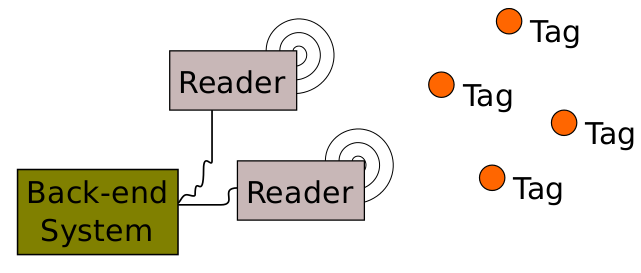
\includegraphics[width=4cm]{img/archRFID}
        \end{tabular}
\end{description}


\subsection{Daily Life Example}

\begin{tabular}{m{6cm}m{6cm}}
	Basic RFID & Evolved RFID\\
		\begin{itemize}
    			\item Pet identification
    			\item Localisation
    			\item Book borrowing and inventories
		\end{itemize} &

	\begin{itemize}
			\item Building Access Control
			\item Payments
			\item Electronic documents
		\end{itemize}
\end{tabular}

	
\subsection{Tags Characteristics}
\begin{center}
    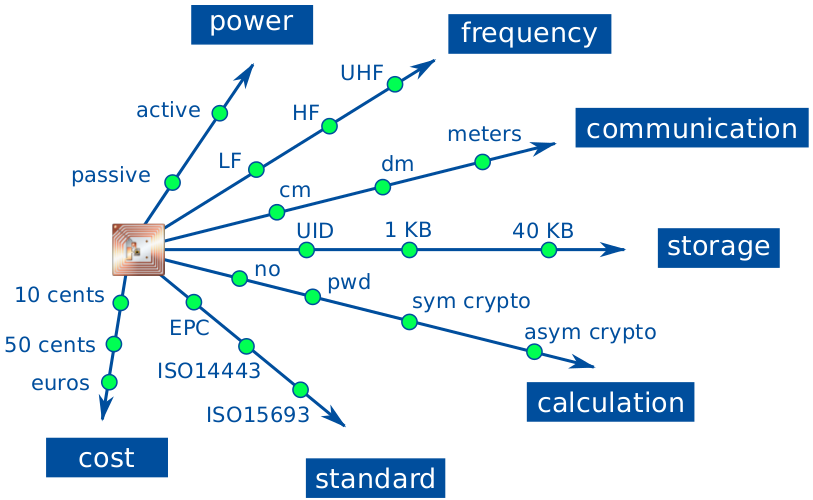
\includegraphics[width=9cm]{img/characRFID}
\end{center}

\subsubsection{Power Source}
\begin{itemize}
    \item \textbf{Passive}:  Tags don't have any internal energy source. They
    get energy from the reader's electromagnetic field.
\item \textbf{Active}:  Tags have a battery that is used both for internal
    calculations and transmission.
\item \textbf{Semi-Passive}:  Tags only have energy for the calculation.
\end{itemize}


\subsubsection{Frequency Bands}
\begin{center}
    \begin{tabular}{|c|c|c|}
        \hline
        & Frequency & Range \\
        \hline
        Low Frequency &  124\text{-}135 kHz & centimeters \\
        High Frequency &  13.56 MHz & decimeters \\
        Ultra-High Frequency & 860\text{-}960 MHz & meters \\
        \hline
    \end{tabular}
\end{center}

\begin{itemize}
    \item Skimming: With a stronger power and better antennas, a tag
        can be read at a greater distance (more than 1m for HF).
    \item Eavesdropping: Reader-to-tag channel (\textbf{forward}) can be
        generally read at a distance greater than tag-to-reader channel
        (\textbf{backward}). (True for \textsc{ISO-14443A}, but false
        for \textsc{ISO-14443B})
\end{itemize}

\subsubsection{Memory}
\begin{itemize}
    \item Tags have at least a few bits to store unique identifier
        \textbf{UID} (32 to 128bits) usually chosen by the manufacturer
        and cannot be changed by the user.
    \item \textbf{EEPROM}, additional memory, can be added: 1KB usually
        to 70KB for passport
\end{itemize}

\paragraph{Note :} Do not use \textbf{UID} for access control because
it can be simulated in a communication.

\subsubsection{Security}

\begin{description}
    \item[Tamper-resistance] A device is tamper-resistant if no adversary can
    get access to its protected memory by use of side-channel attacks.
    \item[Side-channel attack] An attack where the information is
        retrieved from physical implementation of a system. For example,
        (1)~Timing attack, (2)~physical attack, (3)~power analysis
        attacks, (4)~fault injection attacks, ...).
\end{description}

\paragraph{Computation Capabilities}
\begin{itemize}
    \item No computation capabilities, only memory
    \item Simple logic operation
    \item Symmetric cryptography (DES, AES) and microprocessor not
        necessarily required. $\Rightarrow$ LF and HF
    \item Asymmetric cryptographic with microprocessor.
        $\Rightarrow$ HF only currently
\end{itemize}

\subsubsection{Object Name Service}
 The Object Name Service allows to discorver information about a product and related
 service. It allows for object (in this case tag) to communicate with device connected to 
 a network. Each tag own an EPC identifer.
%TODO slide 82 ONS

\paragraph{Near Field Communication (NFC)}
NFC is an extension of RFID, its main difference its that it offer
Peer-to-Peer connections between two (active) devices. NFC Data are exchanged
in a different format.


\subsection{Communication with Tag \textsc{ISO-7816} compliant}

\subsubsection{Memory}
    Internal structure composed of two type of files:
\begin{itemize}
    \item Dedicated File (\textbf{DF})
    \item Elementary File (\textbf{EF}) that can be identified in two subtypes
    \begin{description}
        \item[Internal] Store information used by the card for management and
        control purpose.
        \item[External] Store information used exclusively by the outside world
    \end{description}
    
    \paragraph{Data}
    Data inside an EF is stored in different formats:
    \begin{description}
        \item \textbf{data unit}:  Smallest set of bits which can be unambiguously
            referenced. Default value is 1 byte.
        \item \textbf{record}:  String of bytes which can be handled as a whole. Record
            can be referenced by an 8-bit identifier.
        \item \textbf{data object}:  Structure of information which consists of a tag, a
            length and a value.
    \end{description}
\end{itemize}

\paragraph{Note} The Master File (\textbf{MF}) is a special \textbf{DF}
and is the only mandatory file. Each application is stored in a distinct
\textbf{DF}.

\begin{center}
    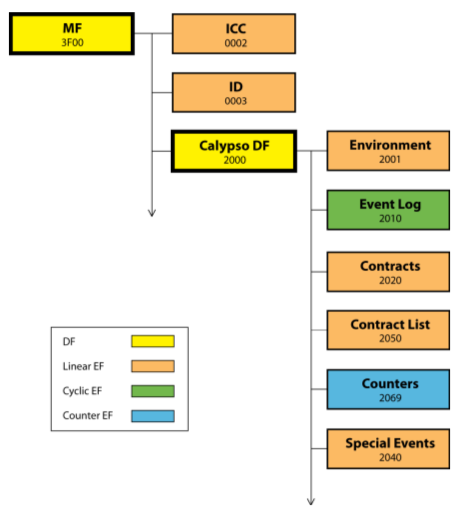
\includegraphics[width=6cm]{img/7816}
\end{center}

\subsubsection{APDU}
Application Protocol Data Unit : CLAss,INStruction,Param1,Param2,Length + Data
\begin{itemize}
	\item Class = Indicates the type of command (interindustry or proprietary)
	\item Instruction = Indicate the specific command (ex:write data)
	\item Param1-2 = Parameter used by the instruction (ex:file and offset)
	\item Length +data

\end{itemize}


\paragraph{Communication}
The protocol used to exchange data is the Application Protocol Data Unit.




\section{Basic of Cryptography}
\subsection{Terminology}
\subsubsection{Definition}
\begin{description}
    \item[Cryptography] Science that design algorithms to ensure
        confidentiality, authentication and Integrity of communication
        through insecure channels.
    \item[Confidentiality] Insurance that a given information cannot be accessed
        by unauthorized parties.
    \item[Cryptanalysis] Science that proves or disproves the security of
        cryptographic algorithm.
    \item[Break cryptographic algorithm] means either:
        \begin{itemize}
            \item Decrypting an encrypted message.
            \item Recovering the key of the cryptographic algorithm.
            \item Proving that a algorithm is less secure than what is claimed.
        \end{itemize}
    \item[Cryptology] Science of cryptography and Cryptanalysis.
\end{description}

\subsubsection{Attacker Model}
\begin{itemize}
    \item \textbf{Passive} adversary: ciphertext-only or known-plaintext
    \item \textbf{Active} adversary: chosen-plaintext or chosen-ciphertext
\end{itemize}

\subsubsection{Encryption Algorithm}
\begin{description}
    \item[Encryption algorithm] Algorithm that transforms an intelligible text
        into text that is unintelligible for non-authorized parties. 

        Usually parametrized with a cryptographic \textbf{key}

    \item[$\Rightarrow$]The input is the plaintext and the output is the ciphertext.
\end{description}


\subsection{Encryption}
%%TODO put it in table


\subsubsection{Cryptographic algorithm categories}
\begin{itemize}
    \item \textbf{Symmetric-key cryptography} where the same key is used for both encryption and
        decryption.

        \begin{itemize}
            \item Based on bit or byte operations.
            \item Tend to be fast.
            \item Typical key-size: 128 bits
            \item Best attack is the exhaustive search.
        \end{itemize}

        \paragraph{Note:} DES is known to not be secure anymore.

        \begin{center}
            \scriptsize
            \begin{tabular}{cc}
                \begin{tikzpicture}
                    \node (P) {Plain};
                    \node [draw, rectangle, right= of P] (E) {Enc};
                    \node [ right= of E] (C) {Cipher};
                    \node [ above= 0.4cm of E] (k) {k};

                    \draw[->] (P) -- (E);
                    \draw[->] (k) -- (E);
                    \draw[->] (E) -- (C);
                \end{tikzpicture}
                &
                \begin{tikzpicture}
                    \node (P) {Cipher};
                    \node [draw, rectangle, right= of P] (E) {Decr};
                    \node [ right= of E] (C) {Plain};
                    \node [ above= 0.4cm of E] (k) {k};

                    \draw[->] (P) -- (E);
                    \draw[->] (k) -- (E);
                    \draw[->] (E) -- (C);
                \end{tikzpicture}
            \end{tabular}
        \end{center}


    \item \textbf{Asymmetric-key cryptography} where there is a public key to encrypt and
        an private key to decrypt.

        \begin{itemize}
            \item Based on mathematical problems
            \item Best attack exploit the mathematical structure.
            \item Typical key size: 1024 bits.
            \item Encryptions and decryptions are slow.
        \end{itemize}

        \paragraph{Certificate:} RSA stands for Rivest-Shamir-Adleman
        Certificate are used to \textbf{identify} of the key owner. A Certificate authority
        issue the certificate.

        \begin{center}
            \scriptsize
            \begin{tabular}{cc}
                \begin{tikzpicture}
                    \node (P) {Plain};
                    \node [draw, rectangle, right= of P] (E) {Enc};
                    \node [ right= of E] (C) {Cipher};
                    \node [ above= 0.4cm of E] (k) {$k_{public}$};

                    \draw[->] (P) -- (E);
                    \draw[->] (k) -- (E);
                    \draw[->] (E) -- (C);
                \end{tikzpicture}
                &
                \begin{tikzpicture}
                    \node (P) {Cipher};
                    \node [draw, rectangle, right= of P] (E) {Decr};
                    \node [ right= of E] (C) {Plain};
                    \node [ above= 0.4cm of E] (k) {$k_{private}$};

                    \draw[->] (P) -- (E);
                    \draw[->] (k) -- (E);
                    \draw[->] (E) -- (C);
                \end{tikzpicture}
            \end{tabular}
        \end{center}

    \item \textbf{Hybrid encryption}: Combine benefits of both symmetric cryptography (speed) and
        asymmetric cryptography (key management).
        $$E_k(m) || E_{k_{pub}}(k)$$
\end{itemize}

\subsubsection{Cypher}
Symmetric-key algorithm can use Block ciphers or Stream ciphers. Block ciphers
acts on the plaintext in blocks. Stream ciphers acts on the plaintext one
symbol at a time.

\begin{center}
    \begin{tabular}{cc}
        Block cipher & Stream cipher\\
        \\
        \scriptsize
        \begin{tikzpicture}
            \node (P) {Block of size $b$};
            \node [draw, rectangle, right= of P] (E) {Algo};
            \node [ right= of E] (C) {Block of size $b$};
            \node [ above= 0.4cm of E] (k) {Key};

            \draw[->] (P) -- (E);
            \draw[->] (k) -- (E);
            \draw[->] (E) -- (C);
        \end{tikzpicture}
        &
        \begin{tikzpicture}
            \node (P) {Plain};
            \node [right= of P] (E) {$\oplus$};
            \node [ right= of E] (C) {Cipher};
            \node [ draw, rectangle, above= 0.4cm of E] (k) {Keystream
            generator};
            \node [left=0.2 of k] (s) {seed};

            \draw[->] (P) -- (E);
            \draw[->] (k) -- (E);
            \draw[->] (E) -- (C);
            \draw[->] (s) -- (k);
        \end{tikzpicture} 
    \end{tabular}
\end{center}

%TODO slide 111

\subsubsection{Key management}
\begin{itemize}
    \item Parties can exchange their key 
        \begin{center}
            \scriptsize
            \begin{tabular}{ccc}
                A & & B \\
                Pick k & \fr{$E_{k_{pub_{B}}}(k)$} & \\
            \end{tabular}
        \end{center}
    \item or agree on shared key by using for example Diffie-Hellman 
        \begin{center}
            \scriptsize
            \begin{tabular}{ccc}
                A & & B \\
                Pick a & \fr{$g^a mod (p)$} & \\
                       & \fl{$g^b mod (p)$} & Pick b\\
                \\
            \multicolumn{3}{l}{Shared key: $g^{ab} mod (p)$}\\
            \end{tabular}
        \end{center}
\end{itemize}


\subsection{Authentication and Integrity}
\begin{itemize}
    \item Entity authentication is asymmetric or symmmetric as
        challenge/response.
    \item Data authentication is
        asymmetric (signature) or symmetric (integrity check) as RSA or
        MAC.
\end{itemize}

\subsection{Hash Function}

$$h:\{0,1\}*\rightarrow\{0,1\}^n$$

\subsubsection{Properties}

\begin{itemize}
    \item \textbf{First preimage resistance}: Given a hash value $y$, it is infeasible to
        find $m$ such that $h(m) = y$.
    \item \textbf{Second preimage resistance}: Given a message $m_1$, it is infeasible
        to find a different message $m_2$ such that $h(m_1)=h(m_2)$.
    \item \textbf{Collision resistance}: It is infeasible to find two different messages
        $m_1$ and $m_2$ such that $h(m_1)=h(m_2)$
    \item \textbf{Random oracle property}: $h(m)$ is distinguishable from a
        random $n$-bit value.
\end{itemize}

\subsubsection{Attacks}
\begin{itemize}
    \item Find a \textit{preimage}: $2^n$
    \item Find \textit{collision}: Thanks to birthday paradox,
        we need about $\sqrt{2^n}$ hash operations to find a
        collision with probability $\frac{1}{2}$

        \paragraph{Birthday Paradox} If we pick $\theta\sqrt{N}$ random numbers,
        independently and uniformly, in {1,2,\ldots,N}, we get at least one number twice
        with probability:
        $$1-e^{-\frac{\theta^2}{2}}$$
\end{itemize}

\subsubsection{Message Authentication Code} 
Hash function that use a key where the naive idea is $h_k(m) = h(k||m)$



\section{Authentication Protocols}
\subsection{Adversary Means}
\begin{itemize}
    \item[Blocks]
\item\textbf{Eavesdropping} Adversary listens to the channel and hopes getting some
        useful data.
    \item\textbf{Skimming} Adversary queries the prover to get some useful information.
    \item\textbf{Modifying} Adversary modifies messages while they transit on the
        channel.
    \item\textbf{Injecting} Adversary injects messages on the channel.
    \item\textbf{Tampering} Adversary obtains content of the protected memory by
        physical means.
    \item\textbf{Exploiting} Adversary obtains information thanks to the system
        implementation.

    \item[Attacks]
    \item\textbf{Re-playing} Adversary replays a message she previously observed.
    \item\textbf{Pre-playing} Adversary skim the prover then plays the message she obtained.
    \item\textbf{Reflecting} Adversary reflects a query from a verifier so that
        answers itself.
    \item\textbf{Guessing} Adversary tries to guess the right answer or key w/o help of
        the prover.
    \item\textbf{Relaying} Adversary forwards the signal between ther verifier and the
        prover.
\end{itemize}

\subsubsection{Dolev-Yao model}
In the \textbf{Dolev-Yao} Model, adversary
is powerful but not all powerful: 
\begin{itemize}
    \item Cannot guess random numbers
    \item Cannot decrypt or create valid ciphertexts without correct secret.
    \item Cannot retrieve private keys from public information.
\end{itemize}

\subsubsection{Avoid replay and preplay}
\begin{itemize}
    \item Authentication based on the exchange of a password or hash of
        password in no secure
    \item[$\Rightarrow$]
        To avoid replay and preplay attack, one-time password or
        challenge/response protocol can be used.
\end{itemize}

\subsection{One-time Passwords}
Passwords are generated with a one-way function $h$.
\begin{enumerate}
	\item Picks a random $S_0$ 
	\begin{center}
	\begin{tikzpicture}
		\node at (0,0) (s0) {$S_0$};
		\node [right =of s0] (s1) {$S_1$};
		\node [right = of s1] (s2) {$S_2$};
		\node [right = of s2] (dots) {\ldots};
		\node [right = of dots] (sn) {$S_n$};
	
		\draw [->]  (s0) -- (s1) node [above,midway] {h};
		\draw [->]  (s1) -- (s2) node [above,midway] {h};
		\draw [->]	(s2) -- (dots) node [above,midway] {h};
		\draw [->]	(dots) -- (sn) node [above,midway] {h};
	\end{tikzpicture}
	\end{center}
	\item Verifier has $S_n$
	\begin{center}
	\begin{tikzpicture}
		\node at (0,0) (p) {P};
		\node [right = 3cm of p] (v) {V};
		
		\draw [->] (p) -- (v) node [above,midway] {$S_n$};
	\end{tikzpicture}
	\end{center}
	\item To authenticate
	\begin{center}
	\begin{tikzpicture}
		\node at (0,0) (p) {P};
		\node [right = 3cm of p] (v) {V};
		
		\draw [->] (p) -- (v) node [above,midway] {$S_{n-1}$};
	\end{tikzpicture} 
	\end{center}
\end{enumerate}
Verifier will check that $h(S_{n-1}) = S_n$, in that case the prover is the
legitimate one. Verifier must update its value to $S_{n-1}$.
\paragraph{Note} A replay attack is not possible because $S_n$ is
updated at every authentication. But a preplay is still possible (depends on the
timing).

\subsection{Challenge response}
Challenge response protocol can use different mechanism:

\begin{enumerate}
    \item Unilateral (only one party is authenticated) authentication
        based on Timestamps where the challenge is based on clock.
    \item Unilateral authentication based on Random Numbers where the
        challenge is based on hash on a
        one time password.
    \item Bilateral (both parties are authenticated) authentication based on Random Numbers
\end{enumerate}

\subsubsection{Challenge Response example}
\begin{itemize}
    \item \textbf{Bad CR} protocol
        \begin{eqnarray*}
            A \leftarrow B & r_B \\
            A \rightarrow B & E_k(r_B) \\
        \end{eqnarray*}

        \begin{itemize}
            \item An attacker can't get the secret key $k$ by
                observing protocol
            \item B can be sure than message comes from A because
                only A and B share $k$
            \item No replay because $r_B$ is a nonce
        \end{itemize}

        \paragraph{Bad}
        \begin{itemize}
            \item Attacker can replay $E_k(r_B)$ if $r_B$ appear twice
            \item If $r_B$ is predictible, the adversary can play
                the role of B (verifier) in front of A, sending him
                a random $r_B$ , then play the role of A (prover) in
                front of B.
            \item Chosen-plaintext attack possible because response
                from A is not randomized.
                \begin{enumerate}
                    \item Adversary can precompute all possible
                        answers
                    \item The adversary can require the
                        prover to sign a chosen value (with
                        public key CR)
                \end{enumerate}
        \end{itemize}

    \item \textbf{Medium CR} protocol
        \begin{eqnarray*}
            A \leftarrow B & r_B \\
            A \rightarrow B & E_k(r_A, r_B) \\
        \end{eqnarray*}

        \paragraph{Bad}
        \begin{itemize}
        \item A adversary can make a reflection attacks
            \begin{enumerate}
                \item Initiate a new protocol with B and send $r_B$
                \item B will response with $E_k(r_B', r_B)$ which is
                    precisely the answer the adversary must provide
                    to B to impersonate A
            \end{enumerate}
        \end{itemize}

    \item \textbf{Better CR} protocol
        \begin{eqnarray*}
            A \leftarrow B & r_B \\
            A \rightarrow B & E_k(r_A, r_B, B) \\
        \end{eqnarray*}

        \begin{itemize}
            \item Unilateral authentication protocol (A to B)
        \end{itemize}

    \item \textbf{Little Better CR} protocol
        \begin{eqnarray*}
            A \leftarrow B & r_B \\
            A \rightarrow B & E_k(r_B, B), r_A \\
            A \leftarrow B & E_k(r_A, A) \\
        \end{eqnarray*}
        
         \begin{itemize}
            \item This is an unilateral authentication applied twice, instead of a mutual
            authentication.
            \item B authenticated A and vice-versa.
            \item Depending of the implementation, B could not know wheter A
            authenticated it  (the two protocols are no linked)
        \end{itemize}
        
	\item \textbf{King CR} protocol
		\begin{eqnarray*}
			A \leftarrow B & r_B \\
			A \rightarrow B & E_k(r_B,r_A, B) \\
			A \leftarrow B & E_k(r_B,r_A,A) \\
		\end{eqnarray*}
\end{itemize}


\subsection{ISO 9798 Challenge/Response}
\begin{itemize}
    \item Mechanism~1: Unilateral authentication with timestamps
    \item Mechanism~2: Unilateral authentication with random numbers
    \item Mechanism~3: Mutual authentication with random numbers
\end{itemize}

\subsubsection{ISO 9798\text{-}2 based on Symmetric-Key Encryption}
\begin{eqnarray*}
    Mechanism~1 \quad & A  \rightarrow B &  E_k(t_A,B)\\
    \\
    Mechanism~2 \quad & A \leftarrow  B & r_B \\
                & A  \rightarrow B & E_k(r_B,B) \\
    \\
    Mechanism~3 \quad & A  \leftarrow B & r_B \\
                & A  \rightarrow B & E_k(r_A,r_B,B) \\
                & A  \leftarrow  B & E_k(r_B,r_A) \\
    \\
    Map1 \quad & A  \leftarrow B & r_B \\
                & A  \rightarrow B & E_k(A, B, r_B,r_A) \\
                & A  \leftarrow  B & E_k(\textcolor{red}{B},r_A) \\
    \\
    Map1.1 \quad & A  \leftarrow B & r_B \\
                & A  \rightarrow B & E_k(A, B, r_B,r_A) \\
                & A  \leftarrow  B & E_k(r_A) 
\end{eqnarray*}

\subsubsection{ISO 9798\text{-}4 based on Hash function}
\begin{eqnarray*}
    Mechanism~1 \quad & A \rightarrow B & H_k(t_A,B),t_A \\
    \\
    Mechanism~2 \quad & A \leftarrow B & r_B \\
                      & A \rightarrow B & H_k(r_B,B),B \\
    \\
    Mechanism~3 \quad & A \leftarrow B & r_B \\
                      & A \rightarrow B & H_k(r_A,r_B,B),r_A \\
                      & A \leftarrow B & H_k(r_B,r_A,A) 
\end{eqnarray*}

\subsubsection{ISO 9798\text{-}3 based on Public-Key Signature}
\begin{eqnarray*}
    Mechanism~1 \quad & A \rightarrow B & S_A(t_A,B),B,t_A,cert_A \\
    \\
    Mechanism~2 \quad & A \leftarrow B & r_B\\
                      & A \rightarrow B &
    S_A(r_A,r_B,B),B,r_A,cert_A \\
    \\
    Mechanism~3 \quad & A \leftarrow B & r_B \\
                      & A \rightarrow B &
    S_A(r_A,r_B,B),B,r_A,cert_A \\
    & A \leftarrow B & S_B(r_B, r_A, A), A, cert_B \\
    \\
    Pub-witness & A \leftarrow B & h(r), B, P_A(r, B) \\
    & A \rightarrow B & r \\
    \\
    Public-key & A \leftarrow B & P_A(r_B, B) \\
                                    & A \rightarrow B & P_B(r_B, r_A)\\
                                    & A \leftarrow B & r_A
\end{eqnarray*}

\paragraph{Note} 
\begin{itemize}
    \item $r$ is a witness, it proves that B knows r : this avoids a
        chosen-plaintext attack
    \item $P_A(m)$ means the
        encryption of the message $m$ with A’s public key.
\end{itemize}


\subsection{Authentication with Key Establishment}
During the phase of authentication phase, the two parties can exchange key
material.

\begin{itemize}
    \item The \textbf{session key} is $k_1$ or a key-derivation function  
        $f(k_1,k_2)$ if there is $k_1$ and $k_2$
\end{itemize}

\subsubsection{ISO 11770\text{-}2 Symmetric-Key}
\begin{eqnarray*}
    Mechanism~4 \quad &  A \leftarrow B & r_B \\
                      & A \rightarrow B & E_k(r_B,B,k_1) \\
    \\
    Mechanism~6 \quad & A \leftarrow B & r_B \\
                      & A \rightarrow B & E_k(r_A,r_B,B,k_1) \\
                      & A \leftarrow B & E_k(r_B,r_A,k_2) \\
\end{eqnarray*}

\paragraph{Note}
Mechanism 6 used in basic access control of ePassport

\subsubsection{Nedham\text{-}Schroeder Public-Key}
\begin{eqnarray*}
    Original \quad &  A \leftarrow B & P_A(k_1,B)  \\
                   & A \rightarrow B &  P_B(k_1,k_2) \\
                   & A \leftarrow B & P_A(k_2) \\
    \\
    Modified \quad &  A \leftarrow B & P_A(k_1, B, r_1)  \\
                   & A \rightarrow B & P_B(k_2,r_1,r_2) \\
                   & A \leftarrow B & r_2 \\
\end{eqnarray*}

\subsubsection{ISO 11770\text{-}3 Asymmetric-Key}
\begin{eqnarray*}
    Mechanism~5 \quad &  A \leftarrow B & r_B \\
                      & A \rightarrow B & r_A,r_B,B, \quad P_B(A,k_1),
    \quad S_A(r_A,r_B,B,P_B(A,k_1))\\
    & A \leftarrow B &
    r_B,r_A,A, \quad P_A(B,k_2), \quad S_B,(r_B,r_A,A,P_A(B,k_2))\\
    \\
    Mechanism~6 \quad &  A \leftarrow B & P_A(B,k_2,r_B) \\
                      & A \rightarrow B & P_B(A,k_2,r_B,r_A) \\
                      & A \leftarrow B & r_A 
\end{eqnarray*}

\paragraph{Mechanism~5} 
\begin{itemize} 
        \item Session key can also be only $k_1$ or $k_2$.
In such a case, $P_A(B, k_2)$ can be omitted (resp. $P_B (A, k_1 )$).
\end{itemize}

\paragraph{Mechanism~6}
\begin{itemize}
    \item Only encryption is used (no signature) but required stronger
        encryption scheme
    \item Instead of use $f(k_1, k_2)$, $k_1$ may be used by A to encrypt messages for B and
        authenticate messages from B, and a similarly for $k_2$ .
\end{itemize}

\subsubsection{X.509}
Mutual authentication protocol

\begin{eqnarray*}
    2~Pass \quad &  A \leftarrow B & cert_B,D_B,S_B(D_B) 
                 \quad \textrm{ where } D_B = ( t_B,r_B,A,data*_1,P_A(k_1)*)\\
                 & A \rightarrow B & cert_A,D_A,S_A(D_A) 
                  \quad \textrm{ where  } D_A =
    (t_A,r_A,B,r_B,data_2,P_B(k_2)* )\\
    \\
    3~Pass \quad &  A \leftarrow B & cert_B,D_B,S_B(D_B) 
        \quad \textrm{ where  } D_B = (t_B,r_b,A,data_1,P_A(k_1)*) \\
        & A \rightarrow B & cert_A,D_A,S_A(D_A) 
        \quad \textrm{ where } D_A = (t_A,r_A,B,r_B,data*_2,P_B(k_2)*)
        \\
        & A \leftarrow B & r_A,A,S_B(r_A,A) 
\end{eqnarray*}

\begin{itemize}
    \item $t_x$ defines a validity period 
    \item  $r_x$ includes a sequential component
\end{itemize}

\paragraph{2~Pass} B does not sign any nonce sent by A

\subsection{Conclusion}
\begin{itemize}
    \item Challenge/response protocols are secure when used with care
    \item Because of the reflection attack, it is better to use an
        asymmetric form of the exchange
    \item General idea to get a good scheme: \textbf{2 nonces +
        identities}
\end{itemize}


\section{Example of poor design}
%TODO


\section{Time-memory Trade-off}
\subsection{One-way Function} 

\begin{center}
    Function $h: A \rightarrow B$: 
    \begin{tabular}{l}
        easy to compute \\
        but hard to invert.
    \end{tabular}
\end{center}

One-way function are used to store password. To break password, an exhaustive
search can be used in two different ways.
\begin{table}[ht!]
    \centering
    \begin{tabular}{|c|c|c|}
        \hline
        & Online exhaustive search & Precalculated exhaustive search \\
        \hline
        Computation & $ |A|:=N $ & 0 \\
        Storage & 0 & N \\
        Precalculation & 0 & N \\
        \hline
    \end{tabular}
\end{table}

\subsection{Hellman's TMTO}
Hellman table is used to pre-calculation phase to speed up the online attack.

\subsubsection{Table creation}
%$$ H: A \to B \quad the\ hash\ function $$
%$$ R: B \to A \quad the\ reduction\ function $$
%A number M of chains is generated from a arbitrary value in A\@:

\begin{tabular}{m{6cm}m{8cm}}
    \begin{tikzpicture}
        \node[draw, circle] (A1) {S1};
        \node[draw, circle] (A2) [below=of A1] {};
        \node[draw, circle] (A3) [below=of A2] {};
        \node[draw, circle] (A4) [below=of A3] {E1};

        \node[draw, circle] (B1) [below right=0.5cm and 3cm of A1] {};
        \node[draw, circle] (B2) [below=of B1] {};
        \node[draw, circle] (B3) [below=of B2] {};

        \node [draw, ellipse, fit={(A1) (A2) (A3) (A4)}] (F) {};
        \node [draw, ellipse, fit={(B1) (B2) (B3) }] (FF) {};

        \draw[->] (A1) edge node[above] {h} (B1);
        \draw[->] (B1) edge node[above] {R} (A2);

        \path[->] (A2) edge (B2)
        (B2) edge (A3)
        (A3) edge (B3)
        (B3) edge (A4);

    \end{tikzpicture}
    &
    \begin{itemize}
        \item $h: A \to B$
        \item $R: B \to A$

        \item[$\Rightarrow$] R is the reduction function.
    \end{itemize}
    $$$$
    \begin{tikzpicture}
        \node[draw, circle] (A1) {S1};
        \node[draw, circle] (A2) [right=of A1] {};
        \node[draw, circle] (A3) [right=of A2] {};
        \node[draw, circle] (A4) [right=of A3] {};

        \node[draw, circle] (A5) [right=of A4] {};
        \node[draw, circle] (A6) [right=of A5] {};
        \node[draw, circle] (A7) [right=of A6] {E1};

        \path[bend left, ->] (A1) edge node[above] {h} (A2)
        (A2) edge node[above] {R} (A3)
        (A3) edge node[above] {h} (A4)

        (A5) edge node[above] {h} (A6)
        (A6) edge node[above] {R} (A7);

        \node[draw, circle] (B1) [below=of A1] {S2};
        \node[draw, circle] (B2) [right=of B1] {};
        \node[draw, circle] (B3) [right=of B2] {};
        \node[draw, circle] (B4) [right=of B3] {};

        \node[draw, circle] (B5) [right=of B4] {};
        \node[draw, circle] (B6) [right=of B5] {};
        \node[draw, circle] (B7) [right=of B6] {E2};

        \path[bend left, ->] (B1) edge node[above] {h} (B2)
        (B2) edge node[above] {R} (B3)
        (B3) edge node[above] {h} (B4)

        (B5) edge node[above] {h} (B6)
        (B6) edge node[above] {R} (B7);

    \end{tikzpicture}
    \\
\end{tabular}

During the generation of the chains, chains may collide between each other, to
avoid that, different reduction function must be used.
\subsubsection{Online attack}
%%TODO ADD from the book, image
The idea is to take the a value $h$ in B, use the reduction function to get in A
and check if the value is contains in the last column of the table match.
If they don't match, use two reduction function and redo the verification.
If the verification fails, redo with 3 reduction function and so on.\ if
no match is found then the attack fails.

When there is a match, redo the chains from the beginning and stop when the
current value is equal to $h$. The password is the value just before $h$
%%TODO false alarms

\subsection{Oechslin Tables}
Oechslin tables also called rainbow table. The main difference compared to
Hellman table is that it uses different reduction function per column such that:

\begin{itemize}
    \item If 2 chains collide in different columns, they don't merge.
    \item If 2 chains collide in same column, merge can be detected.
\end{itemize}

\paragraph{Theorem} The success probability of a table is bounded:
\begin{itemize}
    \item
        Given $t$ and a sufficiently large $N$, the expected maximum number of
        chains per perfect rainbow table without merge is:
        $$ m_{\max}(t)\approx\frac{2N}{t+1} $$
    \item
        Given $t$, for any problem of size $N$, the expected maximum probability of
        success of a single perfect rainbow table is:
        $$ P_{\max}(t)\approx 1 - (1-\frac{2}{t+1})^t $$
        which tends toward $ 1 - e^{-2}\approx 86\% $ when $t$ is large.

        %%TODO have we seen that Average cryptanalysis time ?
\end{itemize}



\section{Generating Randomness}
\subsection{Introduction}
\begin{description}
    \item[Random Numbers] Random numbers are sequence of statistically
        independent and unbiased numbers.
    \item[Random Bits] Random bits are a sequence of statistically independent
        and unbiased binary digits.
    \item[Uniform distribution] All the numbers in a given range must occur
        equally often.
    \item[Independence] Given the knowledge of the all previous numbers
        generated, you can not predict the next number.
\end{description}

\subsubsection{Entropy}
The entropy is used to describe a measure of randomness, a description
of how hard a value is to guess.

\begin{itemize}
    \item Let us assume that $X$ is a discrete random variable on the sample
        space $ \Omega_n = \{\omega_1,\omega_2,\ldots,\omega_n\} $ with the
        probability distribution $P=\{ p_i,1 \leq i \leq n \}$. The entropy $H(X)$
        of X is defined by:
        $$ H(X)= - \sum_{i=1}^{n} p_i \log_{2}p_i $$
\end{itemize}

\subsubsection{Kolmogorov}
The idea of Kolmogorov is to measure the randomness with the
complexity of the minimal program (Turing machine) that
generates a sequence

\subsubsection{Common Uses} 
\begin{itemize} 
    \item Randomness is needed for key generation, nonces, salt,\ldots
    \item[Note] A random number can do the job of an arbitrary number. The
        reverse is not true
\end{itemize}

\subsection{Generating Randomness}
\begin{description}
    \item[Random bit Generator] A random bit generator is a device or algorithm
        which outputs a sequence of statistically independent and unbiased binary
        digits.

        \begin{itemize}
            \item[$\Rightarrow$] A random integer in the interval [0;n] can be obtained by
                generating a random bit sequence of length $ \lfloor \log{}{n} \rfloor + 1 $
                and converting it to an integer.
        \end{itemize}
\end{description}

\begin{center}
    \textit{Anyone who attempts to generate random numbers by
    deterministic (predictable, reproducible) means is, of course, living in a state of sin.}
\end{center}


\subsection{Hardware Random Number Generators}
The source of entropy come the software (time, process ID, user) or the hardware
(mechanical noises, electrical noises).

\subsubsection{Random Number Generators}
\begin{tabular}{m{13cm}m{3cm}}
    \begin{itemize}
        \item\textbf{Non-deterministic RNGs} (True RNGs): Each bit produced by a HRNG comes
            from the observation of an unpredictable physical process.
        \item\textbf{Deterministic RNGs} (PRNG): Each bit is produced by a deterministic
            algorithm properly initialized.
    \end{itemize}
    &
    \begin{tikzpicture}[node distance=0.5cm]
        \node[draw, rectangle] (A) {TRNG};
        \node[draw, rectangle, below =of A] (C) {PRNG};
        \node[below=of C] (D) {output};

        \path[->] (A) edge (C)
        (C) edge (D);
    \end{tikzpicture}
\end{tabular}

\subsection{PRNGs in Theory}
\begin{description}
    \item[Pseudo Random Bit Generator] A PRBG is a deterministic algorithm
        which given a truly random binary sequence of length $k$, outputs a binary
        sequence of length $l \gg k $ which \textbf{appears} to be random. 
        \begin{center}
            \begin{tikzpicture}[node distance=0.5cm]
                \node[draw, rectangle] (A) {Seed};
                \node[draw, rectangle, right =of A] (C) {PRNG};
                \node[right=of C] (D) {pseudo-random bit sequence};

                \path[->] (A) edge (C)
                (C) edge (D);
            \end{tikzpicture}
        \end{center}

        \begin{itemize}
            \item The output of PRBG is not random as the number of
                possible output sequences is at most a small
                fraction, namely $2^k$, of all possible binary
                sequences of length $l$
        \end{itemize}

    \item[PRNG-FSM] A PRNG is a FSM defined by: $$x_{t+1} = f(x_t)$$ 
        $f$ is the transition function and $x_0$ is the seed.
    \item[Period] The period T of the PRNG is the smallest integer such that:
        $x_{t+T} = x_t$
\end{description}

\subsubsection{Generator method}
\begin{itemize}
    \item \textbf{Middle-square Method}

        \begin{tabular}{m{11cm}m{6cm}}
            To generate a sequence of $n$-digit pseudo-random numbers:
            \begin{enumerate}
                \item A $n$-digit seed is created and squared
                \item Middle $n$ digits of the result are output 
                \item The output is know the seed of the process
            \end{enumerate}
            &
            Example with $n$= 6

            \begin{tikzpicture}[node distance=0.5cm]
            \node (firstseed){\begin{tabular}{c}847209\\seed\end{tabular}};
                \node (result)[below=of
                firstseed]{\begin{tabular}{c}717\textcolor{red}{763089}681\\
                seed$^2$\end{tabular}};
                \node (result2)[below=of result]{763089};

                \draw[->] (firstseed) -- (result);
                \draw[->] (result) -- (result2);
                \draw[->] (result2) -| (+1.5cm, +0cm) |- (firstseed);
            \end{tikzpicture}
        \end{tabular}

        \paragraph{Inconvenients}

        \begin{itemize}
            \item For a generator of n-digits numbers, the period cannot be longer than
                $10^n$.
            \item If the middle n digits are all zeroes, the generator then outputs
                zeroes forever.
            \item If the first half of the middle n digits are all zeroes, the
                subsequent values decrease to zero.
            \item There exists short periods.
        \end{itemize}

    \item \textbf{Linear Congruential Generator} A LCG produces a pseudorandom sequence
        of numbers $x_1,x_2,x_3,\ldots$ according to the linear recurrence:
        $$ x_n = a\times x_{n-1} + b \quad \mod{m}\quad with\ n \geq 1 $$

        The integers $a$ (multiplier), $b$ (increment), and $m$ (modulus) are parameters
        which characterize the generator while $x_0$ is the (secret) seed.

        \begin{itemize}
            \item $m$ defines the maximum possible cycle
                length
            \item $a$ defines the number of cycles 
        \end{itemize}

        \begin{tabular}{m{8cm}m{6cm}}
            $$x_{t+1} = \textcolor{red}{5} x_t \quad mod\quad 13$$
            &
            $$x_{t+1} = \textcolor{red}{6} x_t \quad mod\quad 13$$
            \\

            \begin{scriptsize}
                \begin{tikzpicture}
                    \def \n {4}
                    \def \radius {0.8cm}
                    \def \margin {22} % margin in angles, depends on the radius
                    \foreach \s/\r in {1/12, 2/5, 3/1, 4/8} {
                        \node[draw, circle] at ({360/\n * (\s - 1)}:\radius) {$\r$};
                        \draw[<-, >=latex] 
                        ({360/\n * (\s - 1)+\margin}:\radius) 
                        arc 
                        ({360/\n * (\s - 1)+\margin}:{360/\n * (\s)-\margin}:\radius);
                    }
                \end{tikzpicture}
                \begin{tikzpicture}
                    \def \n {4}
                    \def \radius {0.8cm}
                    \def \margin {22} % margin in angles, depends on the radius
                    \foreach \s/\r in {1/11, 2/10, 3/2, 4/3} {
                        \node[draw, circle] at ({360/\n * (\s - 1)}:\radius) {$\r$};
                        \draw[<-, >=latex] 
                        ({360/\n * (\s - 1)+\margin}:\radius) 
                        arc 
                        ({360/\n * (\s - 1)+\margin}:{360/\n * (\s)-\margin}:\radius);
                    }
                \end{tikzpicture}
                \begin{tikzpicture}
                    \def \n {4}
                    \def \radius {0.8cm}
                    \def \margin {22} % margin in angles, depends on the radius
                    \foreach \s/\r in {1/9, 2/7, 3/4, 4/6} {
                        \node[draw, circle] at ({360/\n * (\s - 1)}:\radius) {$\r$};
                        \draw[<-, >=latex] 
                        ({360/\n * (\s - 1)+\margin}:\radius) 
                        arc 
                        ({360/\n * (\s - 1)+\margin}:{360/\n * (\s)-\margin}:\radius);
                    }
                \end{tikzpicture}


            \end{scriptsize}
            &

            \begin{scriptsize}
                \begin{tikzpicture}
                    \def \n {12}
                    \def \radius {2.0cm}
                    \def \margin {7} % margin in angles, depends on the radius
                    \foreach \s/\r in {1/12, 2/2, 3/9, 4/8, 5/10,
                    6/6, 7/1, 8/11, 9/4, 10/5, 11/4, 12/7} {
                        \node[draw, circle] at ({360/\n * (\s - 1)}:\radius) {$\r$};
                        \draw[<-, >=latex] 
                        ({360/\n * (\s - 1)+\margin}:\radius) 
                        arc 
                        ({360/\n * (\s - 1)+\margin}:{360/\n * (\s)-\margin}:\radius);
                    }
                \end{tikzpicture}
            \end{scriptsize}
        \end{tabular}

        \paragraph{Predictable}
        As LCGs is predictable, they are used for simulation purpose and probabilistic
        algorithms but it's insecure
        for cryptographic purpose!

        $\Rightarrow$ Given a partial output sequence, the remainder of
        the sequence can be reconstructed even if the parameters $a$, $b$,
        and $m$ are unknown.

    \item \textbf{Blum-Blum-Shub Generator}
        \begin{itemize}
            \item Let $m=p\times q$ where 
                \begin{enumerate}
                        \item p and q are both primes congruent to 3 modulo
                4 ($p \equiv 3 mod 4$)
                        \item and $ \gcd{\big(\phi(p)}{\phi(q)\big)} $
                            is small. ($\phi(p) = |\{ n < p \wedge n
                                \textrm{ prime with } p$ )
                            \end{enumerate}
                $$\begin{cases}
                        x_0 & = \textrm{seed}\\
                        x_{n+1} & = x^2_n\ \mod{m}
                        \end{cases}$$
            \item We output the parity bit of $x_n$ $(n>0)$.
        \end{itemize}

        \paragraph{Comment}
        It is always safe to use only the lowest order bit. 
        \begin{itemize}
            \item If you use no more than the $log_2 (log_2 (x_n ))$ low order bits, then predicting
                any additional bits from a sequence generated in this manner is
                provable as hard as factoring $m$. 
            \item As long as the initial $x_0$ is secret,
                you can even make $m$ public if you want.
        \end{itemize}

    \item \textbf{ANSI X9.17}: mostly used PRNG 

        \begin{itemize}
            \item Input: a random (and secret) 64-bit seed $x_0$ and a integer $m$
            \item Output: $m$ pseudo-random 64-bit string $x_1,x_2,\ldots,x_m$
                $$x_{t+1} = E_k\bigg(\underbrace{E_k(time())}_{T_t}
                \quad \oplus \quad \underbrace{E_k(x_t \oplus
                T_t)}_{o_t}\bigg)$$
            \item[Note] that $E_k$ is a DES (E-D-E two-key
                triple-encryption) with key $k$
        \end{itemize}

        ANSI X9.17 is fast but there is no security proof (under
        reasonable assumption) that it's a secure PRNG

    \item \textbf{LFSR}
        \begin{center}
            \begin{tikzpicture}
                \node [shape = rectangle](b3) {$b_3$};
                \node [shape = rectangle, right=of b3] (b2) {$b_2$};
                \node [shape = rectangle, right=of b2] (b1) {$b_1$};
                \node [shape = rectangle, above=0.5cm of b1] (xor) {$\oplus$};
                \node [shape = rectangle, right=of b1] (b0) {$b_0$};
                \node [right=of b0] (c) {\begin{tabular}{c}Add to
                pseudo-\\random sequence\end{tabular}};


                \draw [->] (b3) -- (b2);
                \draw [->] (b2) -- (b1);
                \draw [->] (b1) -- (b0);
                \draw [->] (b1) -- (xor);

                \draw[->] (b0) |- (xor);
                \draw [->] (xor) -| (b3);
                \draw[->] (b0) -- (c);
            \end{tikzpicture}
        \end{center}

\end{itemize}


\subsection{PRNGs in practice}

\subsubsection{Apple Carbon Library}
$$x_{t+1} = 16807 \times x_t \mod 2^{31} -1 $$

\begin{itemize}
    \item Need to be careful with \textbf{overflow}. 
        When you multiply 2 n-bit numbers, the results is on 2n bits.
        \end{itemize}

\subsubsection{UNIX Rand}
$$x_{t+1} = (1103515245 \times x_t) + 12345 \mod 2^{31}$$
\paragraph{Note} This generator is heavily \textbf{biased}!

\begin{lstlisting}[frame=single,language=C]
while(i){
	//set seed to time(NULL), time() return time in ms
	srandom(time(NULL)); 
	//print random number
	printf(''\%d,random()'');
}
\end{lstlisting}
\begin{itemize}
    \item[$\Rightarrow$] If the processor is in GHz , time() will return the
        same value during a certain period of time.
\end{itemize}

%TODO /dev/random /dev/urandom ?

\subsection{Implementation}

A PRNG is roughly defined by 3 functions: \begin{tabular}{ll}
    \texttt{instantiate()} & : defines a unique instance of a PRNG.\\
    \texttt{generate()} & :  produces the random number from the seed.\\
    \texttt{test()} & : tests the randomness of everything.\\
\end{tabular}


\section{Implementation of Hash Functions}

\subsection{Common Hash Functions}
\begin{itemize}
    \item Output size:
    \begin{itemize}
        \item MD5: 128bits
        \item SHA-1: 160 bits
        \item SHA-2: 224/256/384/512 bits
        \item RIPEMD:\@160/128/256/320 bits
        \item Whirlpool: 512 bits
    \end{itemize}
    \item Input size:
    \begin{itemize}
        \item In theory, the size is unlimited but in pratice it is limited
        because the length of the message is concatenated at the end of it and
        follows a predefined format
        \item Internal function with small input size sequentially iterated on
        blocks of messages.
    \end{itemize}
\end{itemize}

\subsection{An insider view}
%%TODO complete
\begin{figure}[ht!]
    \centering
    \begin{tikzpicture}
        \node (input){arbitrary length input};
        \node [shape=rectangle,below =of input](preprocessing){data preprocessing};
        \node [shape=rectangle,below =of preprocessing](compression)
        {compression function};
        \node [shape=rectangle,below =of compression](transformation)
        {optional transformation};
        \node [below =of transformation](output){fixed length output};

        \draw [->] (input) -- (preprocessing);
        \draw [->] (preprocessing) -- (compression);
        \draw [->] (compression) -- (transformation);
        \draw [->] (transformation) -- (output);
    \end{tikzpicture}
\end{figure}

\subsection{Conclusion}
\begin{table}[!h]
    \centering
    \begin{tabular}{c|c|c|c}
        Primitive & Output Length & Legacy & Future \\
        \hline
        SHA-2 & 224,256,384,512 & Yes & Yes \\
        SHA-3 & TBA & Yes & Yes \\
        Whirlpool & 512 & Yes & Yes \\
        \hline
        RIPEMD-160 & 160 & Yes & Yes \\
        SHA-1 & 160 & Yes & No \\
        \hline
        MD-5 & 128 & No & No \\
        RIPEDMD-128 & 128 & No & No \\
    \end{tabular}
\end{table}




\section{Implementation of Block Ciphers}

\subsection{Choice of the Block Cipher}
\begin{center}
    \begin{tabular}{|c|c|c|}
        \hline
        \textbf{Primitive} & \textbf{Legacy} & \textbf{Future} \\
        \hline
        AES & \textcolor{green!50!black}{v} &
        \textcolor{green!50!black}{v} \\
        Camelia & \textcolor{green!50!black}{v} &
        \textcolor{green!50!black}{v} \\
        \hline
        Three-key-3DS & \textcolor{green!50!black}{v} &
        \textcolor{red!50!black}{x} \\
        Two-key-3DS & \textcolor{green!50!black}{v} &
        \textcolor{red!50!black}{x} \\
        Kasumi & \textcolor{green!50!black}{v} &
        \textcolor{red!50!black}{x} \\
        Blowfish & \textcolor{green!50!black}{v} &
        \textcolor{red!50!black}{x} \\
        \hline
        DES & \textcolor{red!50!black}{x} & \textcolor{red!50!black}{x}\\
        \hline
    \end{tabular}
\end{center}

\subsection{Characteristic block cipher}

\subsubsection{Key Generation}
Use a \textbf{good pseudo-random generator (PRG)}.

\paragraph{Poor keys}
Some block ciphers suffer from poor keys. For example DES has 16 known poor
(weak and semi-weak) keys. 

\begin{itemize}
	\item\textbf{Weak keys} : A key $k$ is weak if $\forall m$, $E_k(E_k(m)) = m$
	\item\textbf{Semi-weak keys}: A pair of key $(k_1,k_2)$ is semi-weak if $\forall m$,
	$E_{k_1}(E_{k_2}(m))=m$
\end{itemize}
E is an encryption algorighm.

\subsubsection{Mode of Operation} 
Mode of operation is used to define how to encrypt a message whose length
is larger than the cipher block size.

\begin{center}
    \begin{tabular}{|m{2.5cm}|m{1.5cm}|m{1.5cm}|m{1.5cm}|m{2cm}|m{2.5cm}|}
        \hline
        & \textbf{ECB}        & \textbf{CBC}        & \textbf{CFB}    & \textbf{OFB} & \textbf{Counter} \\
        \hline
        Oriented                   & Block      & Block      & Stream & Stream
        & Stream\\
        Padding                    & Require    & Require    & No & No & No\\
        IV                         & No         & Require    & Require &
        Require & No\\
        \hline
        Decryption done with encryption & No & No & Yes & Yes & Yes \\
        \hline
        Parallelization encryption & Yes        & No         & No &
        Preprocessing if IV know & Preprocessing if nonce/counter know\\
        \hline
        Parallelization decryption & Yes        & Yes        & if IV know &
        Preprocessing if IV know & Preprocessing if nonce/counter know\\
        \hline
    \end{tabular}
\end{center}

\tikzstyle{vertex}=[draw,fill=black!15,circle,minimum size=20pt,inner sep=0pt]
\tikzstyle{encrypt}=[draw,fill=black!15,rectangle,minimum size=20pt,inner sep=0pt]

%TODO: decryption
\begin{itemize}
    \item \textbf{Electronic codeBook (ECB)}: Not suitable for long or strongly structured messages
        \begin{itemize}
            \item Swapping blocks is undetectable
            \item Same plaintext blocks produce same ciphertext blocks
        \end{itemize}


        \begin{tabular}{cm{1.5cm}c}
            $C_n = E_k(M_n)$
            &&
            $M_n = D_k(C_n)$\\
            \\
        \begin{tikzpicture}
            \newcommand{\n}{3}
            \foreach \nr in {1, ..., \n}{
                \node (C\nr) at ({(\nr-\n)*2}, 0) {$C_\nr$};
                \node (M\nr) at ({(\nr-\n)*2}, 2) {$M_\nr$};
                \node (E\nr)[encrypt] at ({(\nr-\n)*2},1) {$E$};
                \node (K\nr) at ({(\nr-\n)*2-1},1) {$K$};

                \draw[->,very thick] (M\nr) -- (E\nr);
                \draw[->,very thick] (K\nr) -- (E\nr);
                \draw[->,very thick] (E\nr) -- (C\nr);
            }
        \end{tikzpicture}
        & &
        \begin{tikzpicture}
            \newcommand{\n}{3}
            \foreach \nr in {1, ..., \n}{
                \node (C\nr) at ({(\nr-\n)*2}, 0) {$M_\nr$};
                \node (M\nr) at ({(\nr-\n)*2}, 2) {$C_\nr$};
                \node (E\nr)[encrypt] at ({(\nr-\n)*2},1) {$D$};
                \node (K\nr) at ({(\nr-\n)*2-1},1) {$K$};

                \draw[->,very thick] (M\nr) -- (E\nr);
                \draw[->,very thick] (K\nr) -- (E\nr);
                \draw[->,very thick] (E\nr) -- (C\nr);
            }
        \end{tikzpicture}
        \end{tabular}

    \item \textbf{Cipher Block chaining (CBC)}: General-purpose block-oriented encryption

        \begin{tabular}{cm{1.5cm}c}
            $C_n = E_k(C_{n-1} \oplus M_{n})$ && 
            $M_n = D_k(C_{n}) \oplus C_{n-1}$ \\
            \\
        \begin{tikzpicture}
            \newcommand{\n}{3}
            \foreach \nr in {1, ..., \n}{
                \node (C\nr)            at ({(\nr-\n)*2},0) {$C_\nr$};
                \node (D\nr)[encrypt]   at ({(\nr-\n)*2},1.5) {$E$};
                \node (x\nr)       at ({(\nr-\n)*2},2.5) {$\oplus$};
                \node (M\nr)            at ({(\nr-\n)*2},3.5) {$M_\nr$};

                \node (K\nr)            at ({(\nr-\n)*2-1},1.5) {$K$};

                \draw[->,very thick] (D\nr) -- (C\nr);
                \draw[->,very thick] (x\nr) -- (D\nr);
                \draw[->,very thick] (M\nr) -- (x\nr);

                \draw[->,very thick] (K\nr) -- (D\nr);
            }

            \foreach \nr in {2, ..., \n}{
                \pgfmathtruncatemacro{\tmp}{\nr-1}
                \draw[->,very thick] ({(\n-\tmp)*-2},0.75) -|
                ({(\n-\tmp)*-2+0.75},0.75) |- ({(\n-\tmp)*-2+0.75},2) |- (x\nr);
            }

            \node (IV) at ({\n*-2+1},2.5) {$IV$};
            \draw[->, very thick] (IV) -- (x1);
        \end{tikzpicture}
        & &
        \begin{tikzpicture}
            \newcommand{\n}{3}
            \foreach \nr in {1, ..., \n}{
                \node (C\nr)            at ({(\nr-\n)*2},0) {$M_\nr$};
                \node (D\nr)[encrypt]   at ({(\nr-\n)*2},2) {$D$};
                \node (x\nr)            at ({(\nr-\n)*2},1) {$\oplus$};
                \node (M\nr)            at ({(\nr-\n)*2},3.5) {$C_\nr$};

                \node (K\nr)            at ({(\nr-\n)*2-1},2) {$K$};

                \draw[->,very thick] (M\nr) -- (D\nr);
                \draw[->,very thick] (D\nr) -- (x\nr);
                \draw[->,very thick] (x\nr) -- (C\nr);

                \draw[->,very thick] (K\nr) -- (D\nr);
            }

            \foreach \nr in {2, ..., \n}{
                \pgfmathtruncatemacro{\tmp}{\nr-1}
                \draw[->,very thick] ({(\n-\tmp)*-2},2.75) -|
                ({(\n-\tmp)*-2+0.75},2.75) |- ({(\n-\tmp)*-2+0.75},2) |- (x\nr);
            }

            \node (IV) at ({\n*-2+1},1) {$IV$};
            \draw[->, very thick] (IV) -- (x1);
        \end{tikzpicture}
        \end{tabular}

    \item \textbf{Cipher feedback (CFB)}: General-purpose stream-oriented encryption

        \begin{tabular}{cm{1.5cm}c}
            $C_n = M_n \oplus E_k(C_{n-1})$ && 
            $M_n = C_n \oplus E_k(C_{n-1})$ \\
            \\
        \begin{tikzpicture}
            \newcommand{\n}{3}
            \foreach \nr in {1, ..., \n}{
                \node (C\nr)            at ({(\nr-\n)*2},0) {$C_\nr$};
                \node (x\nr)   at ({(\nr-\n)*2},1.5) {$\oplus$};
                \node (D\nr)[encrypt]       at ({(\nr-\n)*2-1},1.5) {$E$};
                \node (K\nr)            at ({(\nr-\n)*2-1},2.5) {$K$};
                \node (M\nr)            at ({(\nr-\n)*2},3) {$M_\nr$};

                \draw[->,very thick] (x\nr) -- (C\nr);
                \draw[->,very thick] (M\nr) -- (x\nr);
                \draw[->,very thick] (K\nr) -- (D\nr);
                \draw[->,very thick] (D\nr) -- (x\nr);
            }

            \foreach \nr in {2, ..., \n}{
                \pgfmathtruncatemacro{\tmp}{\nr-1}
                \draw[->,very thick] ({(\n-\tmp)*-2}, 0.75) --
                ({(\n-\nr)*-2-1}, 0.75) -- (D\nr);
            }

            \node (IV) at ({\n*-2+1},0.50) {$IV$};
            \draw[->, very thick] (IV) -- (D1);

        \end{tikzpicture}
        & &
        \begin{tikzpicture}
            \newcommand{\n}{3}
            \foreach \nr in {1, ..., \n}{
                \node (C\nr)            at ({(\nr-\n)*2},0) {$M_\nr$};
                \node (x\nr)            at ({(\nr-\n)*2},1.5) {$\oplus$};
                \node (D\nr)[encrypt]   at ({(\nr-\n)*2-1},1.5) {$E$};
                \node (K\nr)            at ({(\nr-\n)*2-1},0.5) {$K$};
                \node (M\nr)            at ({(\nr-\n)*2},3) {$C_\nr$};

                \draw[->,very thick] (x\nr) -- (C\nr);
                \draw[->,very thick] (M\nr) -- (x\nr);
                \draw[->,very thick] (K\nr) -- (D\nr);
                \draw[->,very thick] (D\nr) -- (x\nr);
            }

            \foreach \nr in {2, ..., \n}{
                \pgfmathtruncatemacro{\tmp}{\nr-1}
                \draw[->,very thick] ({(\n-\tmp)*-2}, 2.4) --
                ({(\n-\nr)*-2-1}, 2.4) -- (D\nr);
            }

            \node (IV) at ({\n*-2+1},2.50) {$IV$};
            \draw[->, very thick] (IV) -- (D1);

        \end{tikzpicture}
        \end{tabular}

    \item \textbf{Output feedback (OFB)}: Enable preprocessing

        \begin{tabular}{cm{1.5cm}c}
            $C_n = M_n \oplus E_k(IV)^n$ && 
            $M_n = C_n \oplus E_k(IV)^n$ \\
            \\
        \begin{tikzpicture}
            \newcommand{\n}{3}
            \foreach \nr in {1, ..., \n}{
                \node (C\nr)            at ({(\nr-\n)*2},0) {$C_\nr$};
                \node (D\nr)   at ({(\nr-\n)*2},1) {$\oplus$};
                \node (x\nr)[encrypt]       at ({(\nr-\n)*2},2.5) {$E$};
                \node (M\nr)            at ({(\nr-\n)*2},3.5) {$K$};

                \node (K\nr)            at ({(\nr-\n)*2-1},1) {$M_\nr$};

                \draw[->,very thick] (D\nr) -- (C\nr);
                \draw[->,very thick] (x\nr) -- (D\nr);
                \draw[->,very thick] (M\nr) -- (x\nr);

                \draw[->,very thick] (K\nr) -- (D\nr);
            }

            \foreach \nr in {2, ..., \n}{
                \pgfmathtruncatemacro{\tmp}{\nr-1}
                \draw[->,very thick] ({(\n-\tmp)*-2},1.75) -|
                ({(\n-\tmp)*-2+0.75},1.75) |- ({(\n-\tmp)*-2+0.75},2) |- (x\nr);
            }

            \node (IV) at ({\n*-2+1},2.5) {$IV$};
            \draw[->, very thick] (IV) -- (x1);

        \end{tikzpicture}
        & &
        \begin{tikzpicture}
            \newcommand{\n}{3}
            \foreach \nr in {1, ..., \n}{
                \node (C\nr)            at ({(\nr-\n)*2},0) {$M_\nr$};
                \node (D\nr)   at ({(\nr-\n)*2},1) {$\oplus$};
                \node (x\nr)[encrypt]       at ({(\nr-\n)*2},2.5) {$E$};
                \node (M\nr)            at ({(\nr-\n)*2},3.5) {$K$};

                \node (K\nr)            at ({(\nr-\n)*2-1},1) {$C_\nr$};

                \draw[->,very thick] (D\nr) -- (C\nr);
                \draw[->,very thick] (x\nr) -- (D\nr);
                \draw[->,very thick] (M\nr) -- (x\nr);

                \draw[->,very thick] (K\nr) -- (D\nr);
            }

            \foreach \nr in {2, ..., \n}{
                \pgfmathtruncatemacro{\tmp}{\nr-1}
                \draw[->,very thick] ({(\n-\tmp)*-2},1.75) -|
                ({(\n-\tmp)*-2+0.75},1.75) |- ({(\n-\tmp)*-2+0.75},2) |- (x\nr);
            }

            \node (IV) at ({\n*-2+1},2.5) {$IV$};
            \draw[->, very thick] (IV) -- (x1);

        \end{tikzpicture}
        \end{tabular}

    \item \textbf{Counter (CTR)}: Enable preprocessing and random access

        \begin{itemize}
            \item Same as OFB but randomizes the encryption with a
                \textbf{counter} value instead of some feedback from previous block
            \item Must have a different counter value for every plaintext block.
        \end{itemize}
        With CTR, a counter value should \textbf{never be used} twice with 
        the same secret key, accross all block of all messages
        \begin{itemize}
        	\item Method 1 : A global counter can be used for all messages, so the
        	counter is never re-initialized (cycling period must be long)
        	\item Method 2 : The counter is reinitialized for every message but a 
        	nonce is append to the counter. 
        \end{itemize}

        \begin{tabular}{cm{1.5cm}c}
            $C_n = M_n \oplus E_k(nonce|counter)$ && 
            $M_n = C_n \oplus E_k(nonce|counter)$ \\
            \\
        \begin{tikzpicture}
            \newcommand{\n}{3}
            \foreach \nr in {1, ..., \n}{
                \node (C\nr)            at ({(\nr-\n)*2},0) {$C_\nr$};
                \node (D\nr)   at ({(\nr-\n)*2},1) {$\oplus$};
                \node (x\nr)[encrypt]       at ({(\nr-\n)*2},2) {$E$};
                \node (M\nr)            at ({(\nr-\n)*2},3) {$nonce||\nr$};

                \node (K\nr)            at ({(\nr-\n)*2-1},1) {$M_\nr$};

                \draw[->,very thick] (D\nr) -- (C\nr);
                \draw[->,very thick] (x\nr) -- (D\nr);
                \draw[->,very thick] (M\nr) -- (x\nr);

                \draw[->,very thick] (K\nr) -- (D\nr);
            }

        \end{tikzpicture}
        & &
        \begin{tikzpicture}
            \newcommand{\n}{3}
            \foreach \nr in {1, ..., \n}{
                \node (C\nr)            at ({(\nr-\n)*2},0) {$M_\nr$};
                \node (D\nr)   at ({(\nr-\n)*2},1) {$\oplus$};
                \node (x\nr)[encrypt]       at ({(\nr-\n)*2},2) {$E$};
                \node (M\nr)            at ({(\nr-\n)*2},3) {$nonce||\nr$};

                \node (K\nr)            at ({(\nr-\n)*2-1},1) {$C_\nr$};

                \draw[->,very thick] (D\nr) -- (C\nr);
                \draw[->,very thick] (x\nr) -- (D\nr);
                \draw[->,very thick] (M\nr) -- (x\nr);

                \draw[->,very thick] (K\nr) -- (D\nr);
            }

        \end{tikzpicture}
        \end{tabular}
\end{itemize}

\subsubsection{Initialization Vector}
\begin{center}
    \begin{tabular}{|m{2.5cm}|m{1.5cm}|m{1.5cm}|m{1.5cm}|}
        \hline
        &  \textbf{CBC}        & \textbf{CFB}    & \textbf{OFB} \\
        \hline
        Confidentiality & No & No & No \\
        \hline
        Integrity & Required & Yes & Yes \\
        \hline
        Freshness & Yes & Yes & Yes\\
        \hline 
        Unpredictability & Required & Not issue & Not issue\\
        \hline
    \end{tabular}
\end{center}

\begin{itemize}
    \item \textbf{Confidentiality}
        Confidentiality is not needed, the IV simply act as a $C_0$, making IV confidential
        $\to$ other cipher block confidential.

    \item \textbf{Integrity}
        If IV is changed, part of the plaintext can be modified. With CBC, you can choose
        what the modified the first plaintext block will be. But CFB and
        OFB, plaintext is random

    \item \textbf{Freshness}
        Freshness must be ensured.
        \begin{itemize}
            \item \textbf{CBC:} If the an IV is used twice (wih same key), then the 2 plaintext
                provide same ciphertext up to the first difference between the two plaintext.

            \item \textbf{CFB:} If IV is used twice and if $M_1,C_1$ is known, then
                $M_2$ can be retrieved (given $C_2$). This true up to the first difference up
                to the first difference between the two plaintext.
                \begin{eqnarray*}
                    C_1 & = & M_1 \oplus E(IV)\\
                    C_2 & = & M_2 \oplus E(IV) \\
                    C_1 \oplus C_2 & = & M_1 \oplus M_2
                \end{eqnarray*}
            \item \textbf{OFB:} Same problem as CFB but all the blocks can be retrieved
                if the IV is used twice.
        \end{itemize}

    \item \textbf{Unpredictability}
        \begin{itemize}
            \item For CFB and OFB, as far as we know predicatbility is not an issue.
            \item With CBC, an adversary who has an idea about the plaintext M can
                use the encryptor as an oracle to check her guess G.
        \end{itemize}
        \begin{center}
            \begin{tabular}{m{4cm}m{8cm}}
                \begin{tikzpicture}
                    \node at (0,0) (xor) {$\oplus$};
                    \node [above = 0.5cm of xor] (msg) {M};
                    \node [left = 0.5cm of xor] (iv) {IV};
                    \node [below = 0.5cm of xor,encrypt] (e) {E};
                    \node [left = 0.5cm of e] (key) {K};
                    \node [below = 0.5cm of e] (cipher) {C};

                    \draw[->,very thick] (iv) -- (xor);
                    \draw[->,very thick] (msg) -- (xor);
                    \draw[->,very thick] (key) -- (e);
                    \draw[->,very thick] (xor) -- (e);
                    \draw[->,very thick] (e) -- (cipher);
                \end{tikzpicture}&
                    \begin{itemize}
                        \item Input : IV,C
                        \item Output : Guess G
                        \item Assumption : Adversary has access
                            to an encryptor oracle.
                    \end{itemize}
                \end{tabular}
            \end{center}
            If the IV is predictable, $IV_G$ is the prediction. Advesary request the oracle
            to encrypt $G\oplus IV \oplus IV_G$
            \begin{align}
                E(G\oplus IV \oplus IV_G) &= E((G\oplus IV \oplus IV_G ) \oplus IV_G) &&\text (CBC\ Mode) \notag\\
                                            &= E(G\oplus IV) \notag
            \end{align}
            If $E(G\oplus IV) = C \to G = M$.

        \item \textbf{IV generation}
            \begin{itemize}
                \item Using a counter ensure freshness
                \item Using a encrypted counter ensure freshness \textbf{and} unpredictability
                    (same key as the one to encrypt message)
            \end{itemize}
    \end{itemize}

\subsubsection{Padding}
\begin{itemize}
    \item Main aim of padding is to fill the last block of plaintext (No
        necessarily the shortest)
    \item Can be either bit vs byte-oriented
    \item Required with ECB and CBC
    \item Padding should be checked after decryption
    \item Padding increases the size of the plaintext
\end{itemize}

\paragraph{Methods}

\begin{itemize}

    \item \textbf{ISO/IEC 9797}
        \begin{itemize}
            \item Method 1: Append some 0-bits (possibly none) to fill
                the last block.
                
                $\Rightarrow$ \textbf{Ambiguous} because trailing 0-bits
                of the message cannot be distinguished from the padding!
        \end{itemize}
                \begin{center}
                    \begin{tabular}{|c|c|c|}
                        \cline{1-1} \cline{3-3}
                        DD DD DD DD DD DD DD DD & & DD DD
                        \textcolor{red!50!black}{00 00 00 00 00 00} \\
                        \cline{1-1} \cline{3-3}
                    \end{tabular}
                \end{center}
        \begin{itemize}
            \item Method 2: Put a 1-bit at the end of the plaintext, then pad with
                some 0-bits (possibly none) to fill the last block of plaintext. 
                
                $\Rightarrow$ To avoid ambiguity, plaintext should
                always be padded even if the last block is already
                completed.
        \end{itemize}
                \begin{center}
                    \begin{tabular}{|c|c|c|}
                        \cline{1-1} \cline{3-3}
                        DD DD DD DD DD DD DD DD & & DD DD
                        \textcolor{green!50!black}{80}
                        \textcolor{red!50!black}{00 00 00 00 00} \\
                        \cline{1-1} \cline{3-3}
                    \end{tabular}
                \end{center}
                $$80_{HEX} = 10000000_{BIN}$$

    \item \textbf{ANSI X9.23}: Append some 0-bits to the message and the
        length (in bytes) of the padding.
                \begin{center}
                    \begin{tabular}{|c|c|c|}
                        \cline{1-1} \cline{3-3}
                        DD DD DD DD DD DD DD DD & & DD DD
                        \textcolor{red!50!black}{00 00 00 00 00}
                        \textcolor{green!50!black}{06}\\
                        \cline{1-1} \cline{3-3}
                    \end{tabular}
                \end{center}

    \item \textbf{ISO/IEC 10126}: Append some random bits to the message
        and the length (in bytes) of the padding.
                \begin{center}
                    \begin{tabular}{|c|c|c|}
                        \cline{1-1} \cline{3-3}
                        DD DD DD DD DD DD DD DD & & DD DD
                        \textcolor{red!50!black}{9F 3B 45 10 23}
                        \textcolor{green!50!black}{06}\\
                        \cline{1-1} \cline{3-3}
                    \end{tabular}
                \end{center}

    \item \textbf{PKCS 7}: Each added byte is the length (in bytes) of the padding.
                \begin{center}
                    \begin{tabular}{|c|c|c|}
                        \cline{1-1} \cline{3-3}
                        DD DD DD DD DD DD DD DD & & DD DD
                        \textcolor{red!50!black}{06 06 06 06 06 06}\\
                        \cline{1-1} \cline{3-3}
                    \end{tabular}
                \end{center}
\end{itemize}

\subsection{Cipher used as Hash Function}
A block cipher can be used in place of a hash function.

\subsubsection{Davies-Meyer} 
$$H_i=E_{m_i}(H_{i-1})\oplus H_{i-1}$$ 

\begin{itemize}
    \item The $m_i$ are blocks of the padded message to be hashed. 
    \item[$\Rightarrow$] This
        construction leads to fixed points $E_m(h)\oplus h=h$.

        The Merkle-Damgard strengthening is used to avoid fixed points: the
        bit-length of the message is appended to its end.
\end{itemize}

\subsubsection{Matyas-Meyer} 
$$H_i = E_{g(H_{i-1})}(m_i)\oplus m_i$$

\begin{itemize}
    \item $m_i$ are blocks of the padded message to be hashed.
    \item Function $g$ is just to map the output size of $H$ into the key size.
\end{itemize}



\section{Implementation of Stream Ciphers}

\subsection{Basics}
\subsubsection{Well-known}
\begin{center}
    \begin{tabular}{|c|c|c|}
        \hline
        Primitive & Legacy & Future\\
        \hline
        Rabbit & \textcolor{green!50!black}{v} & \textcolor{green!50!black}{v}\\
        SNOW3G & \textcolor{green!50!black}{v} & \textcolor{green!50!black}{v}\\
        \hline
        Trivium & \textcolor{green!50!black}{v} &
        \textcolor{red!50!black}{x}\\
        SNOW2.0 & \textcolor{green!50!black}{v} & \textcolor{red!50!black}{x}\\
        \hline
        RC4 & \textcolor{red!50!black}{x} & \textcolor{red!50!black}{x}\\
        A5/1 & \textcolor{red!50!black}{x} & \textcolor{red!50!black}{x}\\
        A5/2 & \textcolor{red!50!black}{x} & \textcolor{red!50!black}{x}\\
        E0 & \textcolor{red!50!black}{x} & \textcolor{red!50!black}{x}\\
        \hline
    \end{tabular}
\end{center}

\subsubsection{One-Time Pad} 
$$C_i = M_i \oplus K_i\quad for\ i=1,2,3,\ldots$$

\begin{tabular}{m{3cm}m{8cm}}
    Key must be:&
\begin{itemize}
    \item generated randomly
    \item at least as long as the message
    \item used once
\end{itemize}
\end{tabular}


\subsubsection{Stream ciphers}
\begin{tabular}{m{2cm}m{14cm}}
    Drawbacks: &
    \begin{itemize}
        \item Key $\neq$ Keystream (keystream is generated
            pseudo-randomly)
        \item Key is shorter than the message
        \item Key must be used \textbf{once}: An IV is appended to the key to
            counter this problem.
    \end{itemize}
\end{tabular}

\begin{center}
    \begin{tikzpicture}[node distance=0.6cm]
    \node [draw, rectangle] (S) {Stream cipher};
    \node [above = of S]  (k) {Secret key};
    \node [right=of S]  (x) {$\oplus$};
    \node [draw, rectangle,above = of x]  (p) {Plaintext};
    \node [draw, rectangle,below=of x]  (c) {Ciphertext};
    \path[->] (k) edge (S)
    (S) edge (x)
    (p) edge (x)
    (x) edge (c);
    \end{tikzpicture}
    \end{center}

As with block ciphers, stream ciphers do not ensure integrity (Associativity
and commutativity)

\paragraph{Modes}
\begin{itemize}
    \item \textbf{Synchronized} mode
    \begin{itemize}
        \item Use a single long stream during the session
        \item A and B initialize the stream with the shared key
        \item A uses the first $|m_A|$ bits of the stream to encrypt message
        $m_A$
        \item B uses the next $|m_B|$ bits of the stream to encrypt message
        $m_B$
        \item A new key must be used for each session.
    \end{itemize}

\item \textbf{Unsynchronized} mode
    \begin{itemize}
        \item The keystream is reinitialized for each new packet
        \item Initialization depends on two inputs k and IV\@.
        \item k secret but constant key
        \item IV non-secret but changing initial vector
    \end{itemize}
\end{itemize}

\subsection{Linear Feedback Shift Registers}
LFSR of length $L$ consists of $L$ stages numbered 0, 1, \ldots, L-1. 
Each stage is capable of storing one bit, having one input, one output and a
clock which controls the movements of data.

\begin{center}
    \begin{tikzpicture}
        \node [shape = rectangle](b3) {$b_{L-1}$};
        \node [shape = rectangle, right=of b3] (b2b) {$\cdots$};
        \node [shape = rectangle, right=of b2b] (b2) {$b_2$};
        \node [shape = rectangle, right=of b2] (b1) {$b_1$};
        \node [shape = rectangle, above=0.7cm of b2] (xor) {$\oplus$};
        \node [shape = rectangle, right=of b1] (b0) {$b_0$};
        \node [right=of b0] (c) {\begin{tabular}{c}Add to
        pseudo-\\random sequence\end{tabular}};


        \draw [->] (b3) -- (b2b);
        \draw [->] (b2b) -- (b2);
        \draw [->] (b2) -- (b1);
        \draw [->] (b1) -- (b0);
        \draw [->] (b1) -- (xor);
        \draw [->] (b2) -- (xor);
        \draw [dotted, ->] (b2b) -- (xor);

        \draw[->] (b0) |- (xor);
        \draw [->] (xor) -| (b3);
        \draw[->] (b0) -- (c);
    \end{tikzpicture}
\end{center}

\subsubsection{At each unit of time}
During each unit of time the following operations are performed:
\begin{enumerate}
    \item Content of stage 0 is outputed and forms part of the output
        sequence.
    \item $\forall_{1 \leq i \leq L-1}$: content of stage $i$ is moved to stage $i-1$ 
    \item Content of stage L-1 is the feedback bit $s_j$ which is
        calculated by adding together modulo 2 the previous contents of a fixed
        subsets of stages 0,1,\ldots,L-1.
\end{enumerate}

\subsubsection{4-bits LFSR example}

\begin{tabular}{m{8cm}m{8cm}}
            \begin{tikzpicture}
                \node [shape = rectangle](b3) {$b_3$};
                \node [shape = rectangle, right=of b3] (b2) {$b_2$};
                \node [shape = rectangle, right=of b2] (b1) {$b_1$};
                \node [shape = rectangle, above=0.5cm of b1] (xor) {$\oplus$};
                \node [shape = rectangle, right=of b1] (b0) {$b_0$};
                \node [right=0.5cm of b0] (c) {\scriptsize\begin{tabular}{c}Add to
                pseudo-\\random sequence\end{tabular}};


                \draw [->] (b3) -- (b2);
                \draw [->] (b2) -- (b1);
                \draw [->] (b1) -- (b0);
                \draw [->] (b1) -- (xor);

                \draw[->] (b0) |- (xor);
                \draw [->] (xor) -| (b3);
                \draw[->] (b0) -- (c);
            \end{tikzpicture}
            &
            If key $1001$ is used as seed, the generated sequence is
                    $$\textcolor{red}{1001}10101111000\textcolor{red}{1001}\cdots$$
        \end{tabular}

\subsubsection{Advantage}
\begin{itemize}
    \item LFSR should never be used by itself as keystreamn generator but they have the advantage of having low implementation costs.
    \item To destroy the linearity:
        \begin{itemize}
            \item A nonlinear combining function on the outputs of several LFSRs
            \begin{center}
                \begin{tikzpicture}[node distance=0.5cm]
            		\node [draw,shape=circle] at (0,0) (func){f};
            		\node [draw,shape=rectangle, left = 1cm of func] (lfsr2) {LFSR2};
                    \node [draw,shape=rectangle,above = of lfsr2] (lfsr1) {LFSR1};
            		\node [right = of func] (keystream) {keystream};
            		\node [below = 0cm of lfsr2] (dot) {\vdots};
            		\node [draw,shape=rectangle, below = 0cm of dot] (lfsrn) {LFSRn};
            		
            		\draw [->] (lfsr1) -- (func);
            		\draw [->] (lfsr2) -- (func);
            		\draw [->] (lfsrn) -- (func);
            		\draw [->] (func) -- (keystream);
            	\end{tikzpicture}
            \end{center}
            \item A nonlinear filtering function on the contents of a single LFSR
            \begin{center}
                \begin{tikzpicture}[node distance=0.6cm]
                \node [shape = rectangle](b3) {$b_3$};
                \node [shape = rectangle, right=of b3] (b2) {$b_2$};
                \node [shape = rectangle, right=of b2] (b1) {$b_1$};
                \node [shape = rectangle, above=0.5cm of b1] (xor) {$\oplus$};
                \node [shape = rectangle, right=of b1] (b0) {$b_0$};
                
                \node [below = 0.5cm of b0] (a) {};
                \node [below = 0.5cm of b1] (b){};
                \node [below = 0.5cm of b2] (c){};
                \node [below = 0.5cm of b3] (d){};
                
                \node [draw,circle, below = of b1] (func) {f};
                \node [right = 1cm of func] (keystream) {keystream};


                \draw [->] (b3) -- (b2);
                \draw [->] (b2) -- (b1);
                \draw [->] (b1) -- (b0);
                \draw [->] (b1) -- (xor);

                \draw[->] (b0) |- (xor);
                \draw [->] (xor) -| (b3);

                
                \draw [->] (b0) -- (func);
                \draw [->] (b1) -- (func);
                \draw [->] (b2) -- (func);
                \draw [->] (b3) -- (func);
                \draw [->] (func) -- (keystream);
            \end{tikzpicture}
            \end{center}
            \item The output of one (or more) LFSRs to control the clock of one
                (or more) other LFSRs.
		\begin{center}
            \begin{tikzpicture}
				\node [draw,shape=circle] (func) {f};
				\node [draw,shape=rectangle, above left =0.3cm and 1cm of func] (lfsrc) {LFSR clocking};
				\node [draw,shape = rectangle, below left = 0.3cm and 1cm of func] (lfsr) {LFSR};
				\node [below right =0.3cm and 3cm of func] (tmp) {output $a_i$};
				\node [above right = 0.3cm and 3cm of func] (tmp1) {discard $a_i$};
				
				\draw [->] (lfsrc) -| (func) node [near start,above] {$s_i$};
				\draw [->] (lfsr) -| (func) node [near start,above] {$a_i$};
				\draw [->] (func) -- (tmp) node [midway,below] {$f(s_i) = 0$};
				\draw [->] (func) -- (tmp1) node [midway,above] {$f(s_i)= 1$};
			\end{tikzpicture}
		\end{center}
        \end{itemize}
\end{itemize}

\subsection{RC4}
Use a secret key of length from 1 to 256 bytes and is efficient in
software.

\begin{itemize}
    \item Array $K$ contains $L$ bytes of key 
    \item $K_i$ denote $K_{(i mod L)}$
    \item Array $S$ always has a permutation of $0, 1, \cdots, N-1$
\end{itemize}
\begin{center}
\begin{tabular}{m{4cm}m{4cm}m{4cm}}
    Initialization & Scrambling & Keystream generation \\
    \begin{lstlisting}[mathescape]
for i in (0 to N-1):
    $S_i$ = i
    \end{lstlisting}
    &
    \begin{lstlisting}[mathescape]
j =0
for i in (0 to N-1):
    j = (j + $S_i$ + $K_i$ ) mod N
    Swap($S_i, S_j$ )
    \end{lstlisting}
    &
    \begin{lstlisting}[mathescape]
i = (i + 1) mod N
j = (j + $S_i$ ) mod N
Swap($S_i , S_j$ )
Output $S_{(S_i +S_j )}$ mod N
\end{lstlisting}
\end{tabular}
\end{center}


\subsection{Conclusion}
Using a stream cipher is tricky \textbf{but} the security of stream ciphers is not
well-established, therefore it should be used carefully.




\section{Implementation of Message Authentication Code}

\subsection{Basics}
The goal of MAC is to prevents tampering with a message. MAC require a secret
key otherwise modification of the message cannot be done. 
\begin{itemize}
    \item[$\Rightarrow$] MAC ensures integrity, authentication but not confidentiality.
\end{itemize}

\subsection{Constructions}
Let $h$ be a hash function, $k$ a key, $m$ the message to be MACed, and $M$ the
computed MAC.
\begin{itemize}
    \item Prefix method: $ M = h(k||m) $
    \item Suffix method: $ M = h(m||k) $
    \item Envelop method:$ M = h(k||p||m||k) $
\end{itemize}

\subsubsection{Hash MAC scheme}
MAC uses hash function rather than block cipher because hash function are
generally faster.

\begin{center}
    \begin{tikzpicture}
        \node [rectangle, red, draw] (H) {h};

        \node [left=1.4cm of H, draw, rectangle] (HMAC) {HMAC(k, m)};

        \node [above=of H, C, o-] (C1) {$||$};
        \node [above right=0.0cm and 0.1cm of C1] (X1) {$\oplus$};
        \node [draw, rectangle,above right=1.4cm and 0.1cm of C1] (k) {$k$};
        \node [draw, rectangle,above left=1.4cm and 0.1cm of C1] (m) {$m$};
        \node [right=0.4cm of X1] (ipad) {\textsc{ipad}};

        \node [right=0.6cm of H, C, o-] (C2) {$||$};
        \node [above right=0.5cm and 1cm of C2] (X2) {$\oplus$};
        \node [left=0.4cm of X2] (opad) {\textsc{opad}};

        \path[->] (H) edge (HMAC)
        (C1) edge (H) 
        (C2) edge (H) 
        (ipad) edge (X1)
        (opad) edge (X2);

        \draw[->] (X2) |- (C2.20);
        \draw[->] (X1) |- (C1);
        \draw[->] (m) |- (C1);
        \draw[] (k.280) edge[->] node (tmp) {} (X1);
        \draw[->] (tmp.center) -| (X2);

        \draw[->] (H) |- (+0.5cm, -0.5cm)  -| (+1.5cm, -0.5cm) |-
        (C2.340);

        \node [below left= 0.4cm and -0.2cm of m] (A) {};
        \node [below = 0.1cm of H] (B) {};
        \node [right = -0.2cm of X2] (C) {};

        \node [draw, double, rectangle, fit={(A) (B) (C) }] (FF) {};
    \end{tikzpicture}
\end{center}

%TODO example 374

\subsubsection{Built upon CBC block-cipher}

It's based on the CBC mode of operation: the \textbf{MAC} is the final
block, intermediary blocks are thrown out and IV consists of zeros.

\begin{itemize}
    \item \textbf{CBC-MAC}

        \begin{tikzpicture}
            \newcommand{\n}{3}
            \foreach \nr in {1, ..., \n}{
                \node (C\nr)            at ({(\nr-\n)*2},0) {};
                \node (D\nr)[encrypt]   at ({(\nr-\n)*2},1.5) {$E$};
                \node (x\nr)       at ({(\nr-\n)*2},2.5) {$\oplus$};
                \node (M\nr)            at ({(\nr-\n)*2},3.5) {$M_\nr$};

                \node (K\nr)            at ({(\nr-\n)*2-1},1.5) {$K$};

                \draw[->,very thick] (x\nr) -- (D\nr);
                \draw[->,very thick] (M\nr) -- (x\nr);

                \draw[->,very thick] (K\nr) -- (D\nr);
            }

            \node (C3)            at ({(3-\n)*2},0) {MAC};

            \foreach \nr in {2, ..., \n}{
                \newcommand{\tmp}{\n-\nr}
                \pgfmathtruncatemacro{\tmp}{\nr-1}
                \draw[->,very thick] (D\tmp) -- ({(\n-\tmp)*-2},0.75) -|
                ({(\n-\tmp)*-2+0.75},0.75) |- ({(\n-\tmp)*-2+0.75},2) |- (x\nr);
            }

            \draw[->,very thick] (D\n) -- (C\n);
            \node (IV) at ({\n*-2+1},2.5) {$0$};
            \draw[->, very thick] (IV) -- (x1);
        \end{tikzpicture}

        \paragraph{Characteristic}
        \begin{itemize}
            \item The IV should not be random
            \item Slower than HMAC
            \item The MAC can be truncated to enforce security but this also reduces the
                key search space
        \end{itemize}

        \paragraph{Security}
        \begin{itemize}
            \item CBC-MAC is secure for messages of a fixed number of blocks assuming
                the block cipher is secure.
            \item Not secure with variable lengths
            \item CBC-MAC $(length(M)||M)$ to avoid truncation attacks
        \end{itemize}

    \item \textbf{Retail-MAC}: the last block is decrypted with key $k'$
        then re-encrypted with $k$. This reduces the threat of exhaustive key search

        \begin{tikzpicture}
            \newcommand{\n}{3}
            \foreach \nr in {1, ..., \n}{
                \node (C\nr)            at ({(\nr-\n)*2},0) {};
                \node (x\nr)       at ({(\nr-\n)*2},2.5) {$\oplus$};
                \node (M\nr)            at ({(\nr-\n)*2},3.5) {$M_\nr$};


                \draw[->,very thick] (x\nr) -- (D\nr);
                \draw[->,very thick] (M\nr) -- (x\nr);

                \draw[->,very thick] (K\nr) -- (D\nr);
            }

            \foreach \nr in {1, ..., 2}{
                \node (K\nr)            at ({(\nr-\n)*2-1},1.5) {$K$};
                \node (D\nr)[encrypt]   at ({(\nr-\n)*2},1.5) {$E$};
            }


                \node (K3)            at ({(3-\n)*2-1},1.5) {$K'$};
            \node (D3)[encrypt]   at ({(3-\n)*2},1.5) {$D$};
            \node (DB3)[encrypt]   at ({(3-\n)*2},0.5) {$E$};
            \node (KB3)   at ({(3-\n)*2+1},0.5) {$K$};

            \node (C3)            at ({(3-\n)*2},-0.5) {MAC};

            \foreach \nr in {2, ..., \n}{
                \newcommand{\tmp}{\n-\nr}
                \pgfmathtruncatemacro{\tmp}{\nr-1}
                \draw[->,very thick] (D\tmp) -- ({(\n-\tmp)*-2},0.75) -|
                ({(\n-\tmp)*-2+0.75},0.75) |- ({(\n-\tmp)*-2+0.75},2) |- (x\nr);
            }

            \draw[->,very thick] (DB\n) -- (C\n);
            \draw[->,very thick] (D\n) -- (DB\n);
            \draw[->,very thick] (KB\n) -- (DB\n);
            \node (IV) at ({\n*-2+1},2.5) {$0$};
            \draw[->, very thick] (IV) -- (x1);
        \end{tikzpicture}

        \begin{itemize}
            \item Encrypt $length(M)$ with K, yielding K' and use it as key for the
                MAC function
        \end{itemize}

    \item \textbf{CMAC}
        %TODO finish CMAC

        \begin{tabular}{cc}
            (a) Multiple of block size & (b) Not multiple of block size
            \\
        \begin{tikzpicture}
            \newcommand{\n}{3}
            \foreach \nr in {1, ..., \n}{
                \node (C\nr)            at ({(\nr-\n)*2},0) {};
                \node (x\nr)       at ({(\nr-\n)*2},2.5) {$\oplus$};
                \node (M\nr)            at ({(\nr-\n)*2},3.5) {$M_\nr$};

                \node (K\nr)            at ({(\nr-\n)*2-1},1.5) {$K$};
                \node (D\nr)[encrypt]   at ({(\nr-\n)*2},1.5) {$E$};

                \draw[->,very thick] (x\nr) -- (D\nr);
                \draw[->,very thick] (M\nr) -- (x\nr);

                \draw[->,very thick] (K\nr) -- (D\nr);
                
            }


            \node (C3)            at ({(3-\n)*2},0) {MAC};
            \node (A) at ({(3-\n)*2+1},2.5) {$K_1$};


            \foreach \nr in {2, ..., \n}{
                \newcommand{\tmp}{\n-\nr}
                \pgfmathtruncatemacro{\tmp}{\nr-1}
                \draw[->,very thick] (D\tmp) -- ({(\n-\tmp)*-2},0.75) -|
                ({(\n-\tmp)*-2+0.75},0.75) |- ({(\n-\tmp)*-2+0.75},2) |- (x\nr);
            }

            \draw[->,very thick] (D\n) -- (C\n);
            \draw[->,very thick] (A) -- (x\n);
            \node (IV) at ({\n*-2+1},2.5) {$0$};
            \draw[->, very thick] (IV) -- (x1);
        \end{tikzpicture}
        &
        \begin{tikzpicture}
            \newcommand{\n}{3}
            \foreach \nr in {1, ..., \n}{
                \node (C\nr)            at ({(\nr-\n)*2},0) {};
                \node (x\nr)       at ({(\nr-\n)*2},2.5) {$\oplus$};
                \node (M\nr)            at ({(\nr-\n)*2},3.5) {$M_\nr$};

                \node (K\nr)            at ({(\nr-\n)*2-1},1.5) {$K$};
                \node (D\nr)[encrypt]   at ({(\nr-\n)*2},1.5) {$E$};

                \draw[->,very thick] (x\nr) -- (D\nr);
                \draw[->,very thick] (M\nr) -- (x\nr);

                \draw[->,very thick] (K\nr) -- (D\nr);
                
            }


            \node (C3)            at ({(3-\n)*2},0) {MAC};
            \node (A) at ({(3-\n)*2+1},2.5) {$K_2$};


            \foreach \nr in {2, ..., \n}{
                \newcommand{\tmp}{\n-\nr}
                \pgfmathtruncatemacro{\tmp}{\nr-1}
                \draw[->,very thick] (D\tmp) -- ({(\n-\tmp)*-2},0.75) -|
                ({(\n-\tmp)*-2+0.75},0.75) |- ({(\n-\tmp)*-2+0.75},2) |- (x\nr);
            }

            \draw[->,very thick] (D\n) -- (C\n);
            \draw[->,very thick] (A) -- (x\n);
            \node (IV) at ({\n*-2+1},2.5) {$0$};
            \draw[->, very thick] (IV) -- (x1);
        \end{tikzpicture}
        \end{tabular}

        \paragraph{Generate subkeys}
        %TODO slide 379

\end{itemize}


\subsection{Encrypt and MAC}
Encryption does not ensure integrity but MAC does, so they must be combined.
From the \textbf{LESS} to the \textbf{STRONGER} security:
\begin{itemize}
    \item $ E_K(M) $
    \item Redundancy-then-Encrypt: $ E_K(M,R(M)) $
    \item Hash-then-Encrypt: $ E_K(M,h(M)) $
    \item Hash and Encrypt: $ E_K(M),h(M) $
    \item MAC and Encrypt: $ E_{h1(K)},MAC_{h2(K)}(M) $ (SSH)
    \item MAC-then-Encrypt: $ E_{h1(K)}(M,MAC_{h2(K)}(M)) $ (SSL)
    \item Encrypt-then-MAC\@: $ E_{h1(K)}(M),MAC_{h2(K)}(E_{h1(k)}(M)) $ (IPSec)
\end{itemize}
\paragraph{Note:} Do not hash concatenation of key and message to get a MAC\@.
Never use the same key for both encryption and MAC\@.


\section{Relay attack}

\subsection{Relay attacks}
\begin{description}
    \item[Relay Attack] A relay attack is a form of man-in-the-middle where the
    adversary manipulates the communication by only relaying the verbatim
    messages between two parties.
    \item[Man-In-The-Middle Attack] A man-in-the-middle (MITM) us a form of
    attack, where the adversary provokes or manipulates the communication
    between two parties. Manipulating the communication means relay, withold, or
    insert messages.
\end{description}

\begin{figure}[ht!]
    \centering
    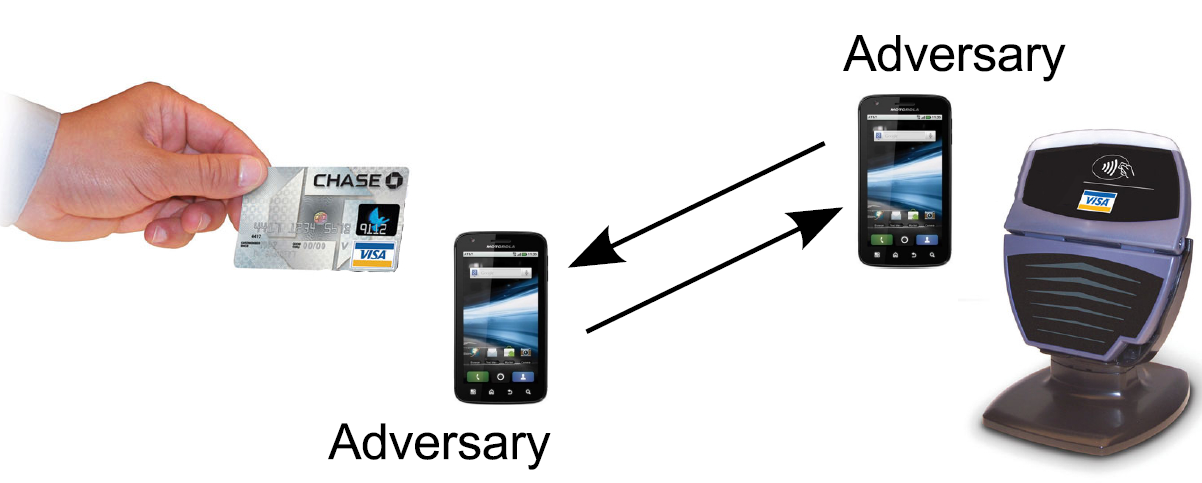
\includegraphics[width=0.7\columnwidth]{img/relay-attack}
\end{figure}
\paragraph{Note:} The do-ability of the Relay attack depends on the timer
between the prover and the verifier. Usually the timer is not tight, by default
its 5ms but it can be extend by the prover.


\begin{description}
    \item[Distance Bounding] A distance bounding is a process whereby one party
    assured:
    \begin{itemize}
        \item Of the identity of a second party,
        \item That the latter is present in the neighborhood of the verifying
        party, at some point in the protocol
    \end{itemize}
\end{description}
\paragraph{Note:} Distance bounding protocol does not avoid relay attacks, if
adversary inside the area of coverage.

Measurement of the distance can be done in different ways:
\begin{itemize}
    \item With the GPS
    \item The strength of the received signal  (RSS)
    \item Round Trip Time (RTT)
\end{itemize}

\subsection{Protocol Analysis}
\begin{description}
    \item[Mafia Fraud] A mafia fraud is an attack where an adversary defeats a
    distance bounding protocol using a man-in-the-middle (MITM) between the
    reader and an honest tag located outside the neighborhood.
    \item[Terrorist Fraud] A terrorist fraud is an attack where an adversart
    defeats a distance bounding protocol using a man-in-the-middle (MITM)
    between the reader and dishonest tag located outside of the neighborhood,
    such that the latter actively helps the adversary to maximize her attack
    success probability, without giving to her any advantage for future attacks
    \item[Distance Fraud] Given a distance bounding protocol, a distance fraud
    is an attack where a dishonest and lonely prover purports to be in the
    neighborhood of the verifier.
\end{description}

%%TODO Hancke and Kuhn's Protocol

\subsection{Comparison with Decision Theory}
%%NOT sure if we have seen this


\section{Privacy}

\subsection{Impact}
Compared to other technologies (video, GSM, \ldots), RFID has several issue
concerning privacy:
\begin{itemize}
    \item Tags cannot be switched-off
    \item Passive tags answer without the agreement of their bearers
    \item Easy to analyze the logs of the readers
    \item Increasing of the communication range
    \item Tags can be almost invisible
\end{itemize}

Privacy issues concerning RFID is being seriously considered by authorites.

\subsection{Classification}

\begin{itemize}
    \item \textbf{Information Meaningful by Itself}: Privacy issues
        appear when the data sent by the tag reveals information
        intrinsic to the marked object or the holder of the object.

        \paragraph{Public transportation}
        MOBIB card are rather powerful RFID tags that embed
        cryptographic mechanisms to avoid impersonation or cloning,
        Personal data are stored in the clear in the card.
        %TODO understand

    \item \textbf{Information Meaningful with the database}: There exist
        website (or technique in general) to make the link between
        anonymous information in database.
\end{itemize}

\subsection{Mitigating the Problem}
\begin{itemize}
    \item Kill command to destroy the tag
    \item Use a faraday cages or a blocker tags to
        avoid clandestine query.
    \item Remove antenna
    \item $\cdots$
\end{itemize}
The problem with these solutions is that they are not convenient.

\subsubsection{Privacy problem}

Nowadays more and more data are collected, it is called
logphilia. But with all these data, information may eventually leak.

The consequence of these information's leakage must be evalutated:
\begin{itemize}
    \item Does all these data need to be store?
    \item Encryption of the sensitive data on the tag in the databases
    \item Authentication for accessing the data
    \item Establishing policies to define who can access the data
\end{itemize}

\subsubsection{Future}
\begin{itemize}
    \item Cryptographic building blocks available in the tags are more
        secure in recent products (lightweight implementation of
        standardized algorithms)
    \item Note that Secure building blocks do not make themselves secure
        applications: 
        \begin{itemize}
            \item The security of the whole application must be considered.
            \item Many SMEs involved in RFID.
        \end{itemize}
\end{itemize}



\section{Biometric Passport}

\subsection{Machine Readable Zone}

\subsubsection{Construction}
\begin{itemize}
    \item An Machine Readable Zone is composed of two lines of 44 characters
    \item Numbers and punctuations not authorized in the name field
    \item Hyphens are replaced by a filler character ('<')
    \item Apostrophes and commas are omitted
    \item First and last names are separated by 2 filler characters
    \item White characters are replaced by filler characters
\end{itemize}

\subsubsection{Check Digits Calculation}
Check digits are computed for each protecfields. They are calculated modulo 10
with continous repetitive weihting of 731
\begin{itemize}
    \item Letters are mapped to their corresponding numerical value:
    A=10, B=11, \ldots, Z=35, '<'=0.
    \item From left to right, each numerical value is multiplied by the weight
    appearing in the same sequential position.
    \item The product of each multiplication is added modulo 10
\end{itemize}

\paragraph{Example} Calculate the check digit of the document number "EH123456<"

\begin{tabular}{m{10cm}m{6cm}}
    \begin{tabular}{|c|c|c|c|c|c|c|c|c|c|}
        \hline
        Number & E & H & 1 & 2 & 3 & 4 & 5 & 6 & < \\
        & 14 & 17 & 1 & 2 & 3 & 4 & 5 & 6 & 0 \\
        \hline
        Weight & 7 & 3 & 1 & 7 & 3 & 1 & 7 & 3 & 1\\
        \hline
        $N\times W \mod{10}$ & 98 & 51 & 1 & 14 & 9 & 4 & 35 & 18 & 0\\
        \hline
    \end{tabular}
    &
    \begin{eqnarray*}
        98+51+1+14+9+4+35+18 &=& 230 \\
        230 \mod 10 &=& 0 
        \end{eqnarray*}
        $\Rightarrow$ The remainder of the division is the check digit $0$.
\end{tabular}

\subsection{DOC 9303}

\begin{center}
    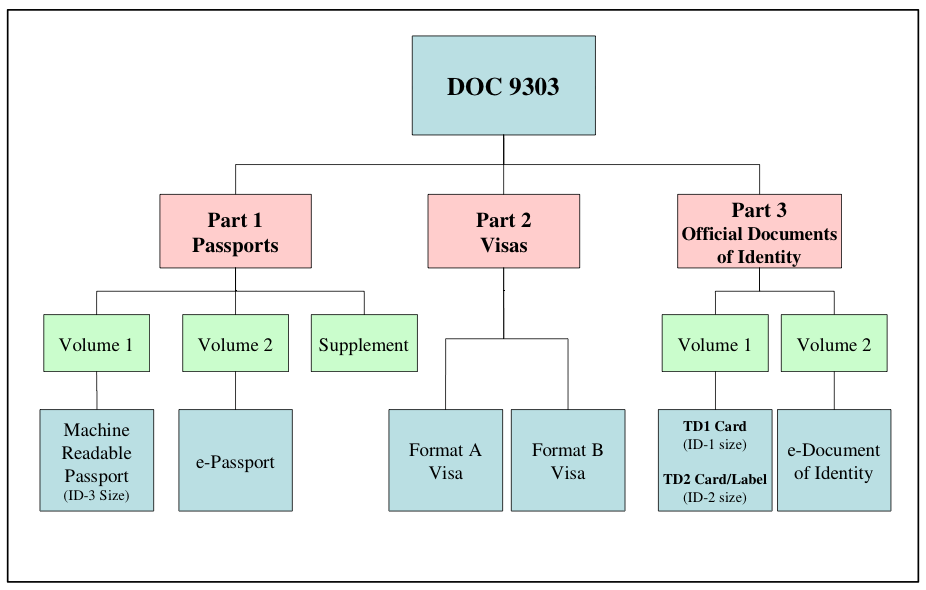
\includegraphics[width=11cm]{img/9303.png}
    \end{center}

\subsubsection{Technical facts about the passport}
\begin{itemize}
    \item Tag is passive (no internal battery)
    \item Tag has a microprocessor (public-key crypto)
    \item Official distance is 10cm
    \item EEPROM capacity: 32KB (minimum)
\end{itemize}

\subsubsection{Passport Content}
\begin{tabular}{|m{2cm}|m{7cm}|m{6cm}|}
    \hline
    Publicly & Publicly possibly after authentication & Never supplied
    by the tag \\
    \hline
    \begin{itemize}
        \item UID 
    \end{itemize}
    &
    \begin{itemize}
        \item Some data groups (DG)
        \item List of data groups on the considered passport (COM)
        \item Cryptographic material signature and hashes (SOD)
    \end{itemize}
    &
    \begin{itemize}
        \item Two symmetric key $K_{ENC},K_{MAC}$ (can be retrieved from MRZ)
        \item One private key $K_{pr}$ (protected memory)
    \end{itemize}
    \\
    \hline
\end{tabular}


\subsection{Protection Mechanisms}
\begin{center}
    \begin{tikzpicture}[node distance= 0.3cm]
        \node [draw=blue, rectangle, text width=5cm] (A) {Modifying data
            of a given passport. Forging a fake passport};

        \node [draw=blue, rectangle, text width=5cm, below=of A] (B) {Cloning a given passport};
        \node [draw=red, rectangle, text width=5cm, below=of B] (C) {Skimming a passport};
        \node [draw=red, rectangle, text width=5cm, below=of C] (D) {Eavesdropping the communication};

        \node [right=2cm of A, text width=4cm] (AA) {Passive Authentication};
        \node [right=2cm of B, text width=4cm] (BB) {Active Authentication};
        \node [right=2cm of C, text width=4cm] (CC) {Basic Access Control};
        \node [right=2cm of D, text width=4cm] (DD) {Secure Messaging};

        \node [right=0cm of AA]  {(Signature)};
        \node [right=0cm of BB]  {(Challenge Response)};
        \node [right=0cm of CC]  {(Reader Authentication)};
        \node [right=0cm of DD]  {(Encryption)};

        \draw[->, >=latex, blue] (AA) to node[] {} (A);
        \draw[->, >=latex, blue] (BB) to node[] {} (B);
        \draw[->, >=latex, red] (CC) to node[] {} (C);
        \draw[->, >=latex, red] (DD) to node[] {} (D);


    \end{tikzpicture}
\end{center}

\subsubsection{Passive Authentication (PA)}
Passive authentication is a \textbf{mandatory security mechanism}: it proves
that the file EF.SOD and LDS are authentic and not modified.

\begin{tabular}{m{8cm}m{7cm}}
    \centering
\begin{tikzpicture}[node distance=0.2cm]
    \node[text width=1.5cm,text centered, rectangle, draw] (1) {$EF.COM$};
    \node[text width=1.5cm,text centered, rectangle, draw, below=of 1] (2) {$DG_1$};
    \node[text width=1.5cm,text centered, rectangle, draw, below=of 2] (3) {$DG_2$};
    \node[text width=1.5cm,text centered,  below=of 3] (4) {$\vdots$};
    \node[text width=1.5cm,text centered, rectangle, draw, below=of 4] (5) {$DG_n$};

    \node[rectangle, draw, dotted, right=0.5cm of 2] (H1) {$hash$};
    \node[rectangle, draw, dotted, right=0.5cm of 3] (H2) {$hash$};
    \node[below=0.5cm of H2] (H3) {$\vdots$};
    \node[rectangle, draw, dotted, right=0.5cm of 5] (H4) {$hash$};

    \node[rectangle, draw,text width=2.5cm, text centered, dotted, right=1cm of H3] (S) {Signature};
    \node[rectangle, draw,text width=2.5cm, text centered, dotted, below =of S] (D) {DS certificate};

    \node[above right=-0.2cm and 1.3cm of H1] (EF) {$EF.SOD$};

    \node [draw, double, rectangle, fit={(H1) (H2) (H3) (H4) (D) (EF) }] (FF) {};

    \node [draw, red, dashed, rectangle, fit={(2) (H1)}] (FF) {};
    \node [draw, red, dashed, rectangle, fit={(3) (H2)}] (FF) {};
    \node [draw, red, dashed, rectangle, fit={(5) (H4)}] (FF) {};
\end{tikzpicture}
& 
\begin{itemize}
    \item \textbf{EF.SOD} contains the hash value of each present
        \textbf{DG}, and signature calculated by the issuing State over values.
    \item The signature can be checked using the Document Signer
        (\textbf{DS}) X.509 certificate. (Available from \textbf{EF.SOD})
    \end{itemize}
\end{tabular}

\begin{itemize}
    \item The DS certificate can be checked using the Country Signing CA (CSCA)
    X.509 cerficate.
    \begin{itemize}
        \item The ICAO PKD does not publish the CSCA certificates
        \item CSCA certificates and revocation lists should be exchanged
        according to bilateral agreements
    \end{itemize}
\end{itemize}

\paragraph{Recommandation} According to DOC 9303:
\begin{itemize}
    \item The passive authentication should use \textsc{RSA},
        \textsc{DSA} or \textsc{ECDSA} for the
    signature schemes
    \item SHA-1, SHA-224/256/384/512 for the hash algorithm
    \item CSCA keys should be renewed every 3-5~years and the DS
    keys every 3~months
\end{itemize}

\subsubsection{Active Authentication (AA)}

The active authentication is an optional security mechanism:
it prove that the \textbf{EF.SOD} belongs to the authentic ePassport, i.e
it is not a cloned one.

\begin{center}
\begin{tabular}{rcl}
    \bf Reader & & \bf ePassport\\
               & \fr{$M_2$} & \\
               & \fl{$Sign(M_2, M_1)$} & \\
    \end{tabular}
\end{center}

\begin{itemize}
    \item Two-pass CR protocol ISO 9796i\text{-}2 Digital Signature Scheme 1
    \item ePassport's public key is stored in DG15
\end{itemize}

The active authentication should rely on RSA, DSA or ECDSA with minimum sizes for
the security parameters should be respectively 1024 bits, 1024 and 160
bits, and 160 bits.

\paragraph{Example with RSA/SHA~1}

\begin{center}
\begin{tabular}{rcl}
    \bf Reader & & \bf ePassport\\
    $M_2 \in_R \{0, 1\}^{64}$   & \fr{$M_2$} & $M_1 \in_R \{0, 1\}^{848}$ \\
                                & & $F = 6A||M_1||SHA1(M_1, M_2)||BC$\\
    $F^* = RSA_{PK_{DG15}}(S)$ &\fl{$S$} & $S = RSA_{SK_{DG15}}(F)$ \\
    $6A||M_1^*||H^*||T^* = F^*$ & & \\
    $SHA1(M_1^*||M_2) ?=? H^*$ &&\\
    \end{tabular}
\end{center}

\subsubsection{Basic Access Control (BAC) and Secure Messaging (SM)}

\begin{tikzpicture}
    \footnotesize
    \node (BAC) {\bf Basic Access Control};
\node[below=0cm of BAC, text width=3.3cm] (BAC1) {\begin{tabular}{l}Encryption Key\\ MAC Key\end{tabular}};

        \node[below=2cm of BAC] (SM) {\bf Secure Messaging};
    \node[below=0cm of SM, text width=3.3cm] (SM1) {\begin{tabular}{l}Session Encryption
    Key\\ Session MAC Key\end{tabular}};

    \node[draw, rectangle, above left=0.0cm and 1.5cm of BAC] (MRZ) {\begin{tabular}{l} Passport
        Number\\Expiration Date \\ Birth Date\end{tabular}};
    \node[above=0cm of MRZ] {\bf MRZ};

    \node[draw, rectangle, double, fit={(BAC) (BAC1)}] (BBAC)  {};
    \node[draw, rectangle, double, fit={(SM) (SM1)}] (SSM)  {};

    \draw[->] (MRZ) -| (BBAC);
    \draw[->] (BBAC) -| (-2.5cm, -1.5cm) |- (SSM);

    \node[above left=0.2cm and 1cm of SM] {$K_r, K_p$};

    \node[right=of BBAC] {\scriptsize \begin{tabular}{rcl}
            \bf Reader &&\bf Passport\\
                       &\fl{$C_p$}&\\
                       &\fr{$a = ENC\big(C_p, C_r, K_r\big), MAC(a)$}&\\
                       &\fl{$b = ENC\big(C_p, C_r, K_p\big), MAC(b)$}&\\
            \end{tabular} };

    \node[right=of SSM] {\scriptsize \begin{tabular}{rcl}
            \bf Reader &&\bf Passport\\
                       &\fr{Authenticated Query}&\\
                       &\fr{Encrypted Data}&\\
            \end{tabular} };
\end{tikzpicture}

\begin{itemize}
    \item Three-pass CR protocol according to ISO 11770\text{-}2 Key Establishment
    Mechanism 6, 2-key 3DES as block cipher
    \item Nonces should be 8-byte long
    \item Encryption done using 3DES in CBC mode with zero-IV according to
    ISO 11568\text{-}2
    \item A cryptographic checksum is calculated over: ISO 9797\text{-}1 MAC
    Algorithm 3 (i.e Retail-MAC), based on DES, zero-IV, ISO 9797\text{-}1 Padding
    Method 2
    \item Encryption and MAC keys derived from the MRZ using SHA-1
\end{itemize}

\begin{tabular}{m{3cm}m{11cm}}
\textbf{Key Derivation} &
\begin{enumerate}
    \item Set $ K_{seed} = trunc_{16}(SHA-1(MRZ\_info))\quad or\ (K_r \oplus K_p)$
    \item Set $ D = K_{seed}||00000001 $
    \item Compute $ H = SHA-1(D) $
    \item First 16 bytes of H are set to the 2-key 3DES $ K_{ENC} $
    \item Set $ D = K_{seed}||00000002 $
    \item Compute $ H = SHA-1(D) $
    \item First 16 bytes of H are set to the 2 DES keys $K_{MAC} $
    \item Adjust the parity bits of the DES keys
\end{enumerate}
\end{tabular}

\subsection{Weaknesses}
BAC keys are derived from the MRZ, especially date of birth, date of expiry,
passport number. 

$\Rightarrow$ But passport numbers are usually not random, DOB and DOE are
neither random.

\begin{itemize}
    \item Relay Attacks: Passport is based on ISO 14443, so it can require to
    increase the timeouts.
    \item Evidence of Presence: Abuse the active authentication which can be
    doable without passing the BAC
    \item Chain of Trust: If the root certificate cannot be verified, making a
    fake passport is quite easy
\end{itemize}

\subsubsection{Information leakage through side channel}
An adversary can guess the issuing state of an ePassport without
knowledge of the BAC keys:
\begin{enumerate}
    \item Send wrong messages to the passport
    \item Analyze the error messages.
    \item  Fingerprint the countries.
\end{enumerate}
Error messages are the external signal of an internal behavior.
Implementer have too frequently to deal themselves with the
error messages but they are not aware of potential security issues.

\subsection{Extended Access Control (EAC)}
EAC is an improved security mechanism that aims to eventually
replace BAC and AA.

\begin{itemize}
    \item Includes the tag authentication (should eventually replace AA)
        and the terminal authentication (makes obsolete BAC because
        only authorized readers have access to the data).
\end{itemize}



\end{document}
